% ============================================================================
% MASGym: A Co-Evolving Red/Blue Security Gym for Multi-Agent LLM Systems.
% AAMAS 2027 submission format (official `aamas' class, anonymous).
%
% The appendices live in a SEPARATE PDF (main_supplement.tex) because only
% bibliographic reference pages are exempt from the 8-page limit.
%
% BUILD:   build_all.bat   (recommended: builds main.pdf then main_supplement.pdf)
%          or: pdflatex main; bibtex main; pdflatex main; pdflatex main
%
% PAGE LIMIT: main track papers are at most EIGHT (8) pages, with any number
% of additional pages for bibliographic references. Do NOT modify style/layout
% parameters. For camera-ready, drop the `anonymous' option and fill in
% author/affiliation/email.
% ============================================================================
% ============================================================================
% Claim the root role before pulling in the preamble: this file holds no
% \documentclass (that lives in preamble.tex), so without this stamp preamble.tex
% would assume it had been selected as Overleaf's Main document and redirect
% back here, re-entering this file.
\makeatletter\def\@masgym@root{main.tex}\makeatother
% ============================================================================
% Shared preamble for BOTH documents:
%   main.tex            -- the 8-page main-track paper
%   main_supplement.tex -- the separate supplementary PDF
%
% Kept in one file so theorem environments, notation macros, and title metadata
% cannot drift between the paper and its supplement. xr is loaded here (inert
% unless \externaldocument is called) so the supplement can resolve the ~57
% main-body cross-references it makes.
% ============================================================================
% ============================================================================
% ---- Overleaf root guard (packaging only; inert when main.tex is the root) --
% Overleaf auto-selects as "Main document" whichever file contains
% \documentclass -- which here is THIS file, not main.tex. Chosen as the root,
% preamble.tex has no \begin{document}/\end{document} and the run dies with
% "! Emergency stop / job aborted, no legal \end found".
%
% So: if nobody claimed us as the root, delegate to main.tex. main.tex stamps
% \@masgym@root before \input us, so when it IS the root this file loads as an
% ordinary preamble and the class is loaded exactly once.
%
% NOTE: any OTHER document that \inputs this preamble (e.g. the supplement's
% main_supplement.tex) must also stamp \@masgym@root, or it will be redirected
% to main.tex.
\makeatletter
\@ifundefined{@masgym@root}{%
  \typeout{MASGym: preamble.tex cannot be a root file -- delegating to main.tex}
  % ============================================================================
% MASGym: A Co-Evolving Red/Blue Security Gym for Multi-Agent LLM Systems.
% AAMAS 2027 submission format (official `aamas' class, anonymous).
%
% The appendices live in a SEPARATE PDF (main_supplement.tex) because only
% bibliographic reference pages are exempt from the 8-page limit.
%
% BUILD:   build_all.bat   (recommended: builds main.pdf then main_supplement.pdf)
%          or: pdflatex main; bibtex main; pdflatex main; pdflatex main
%
% PAGE LIMIT: main track papers are at most EIGHT (8) pages, with any number
% of additional pages for bibliographic references. Do NOT modify style/layout
% parameters. For camera-ready, drop the `anonymous' option and fill in
% author/affiliation/email.
% ============================================================================
% ============================================================================
% Claim the root role before pulling in the preamble: this file holds no
% \documentclass (that lives in preamble.tex), so without this stamp preamble.tex
% would assume it had been selected as Overleaf's Main document and redirect
% back here, re-entering this file.
\makeatletter\def\@masgym@root{main.tex}\makeatother
% ============================================================================
% Shared preamble for BOTH documents:
%   main.tex            -- the 8-page main-track paper
%   main_supplement.tex -- the separate supplementary PDF
%
% Kept in one file so theorem environments, notation macros, and title metadata
% cannot drift between the paper and its supplement. xr is loaded here (inert
% unless \externaldocument is called) so the supplement can resolve the ~57
% main-body cross-references it makes.
% ============================================================================
% ============================================================================
% ---- Overleaf root guard (packaging only; inert when main.tex is the root) --
% Overleaf auto-selects as "Main document" whichever file contains
% \documentclass -- which here is THIS file, not main.tex. Chosen as the root,
% preamble.tex has no \begin{document}/\end{document} and the run dies with
% "! Emergency stop / job aborted, no legal \end found".
%
% So: if nobody claimed us as the root, delegate to main.tex. main.tex stamps
% \@masgym@root before \input us, so when it IS the root this file loads as an
% ordinary preamble and the class is loaded exactly once.
%
% NOTE: any OTHER document that \inputs this preamble (e.g. the supplement's
% main_supplement.tex) must also stamp \@masgym@root, or it will be redirected
% to main.tex.
\makeatletter
\@ifundefined{@masgym@root}{%
  \typeout{MASGym: preamble.tex cannot be a root file -- delegating to main.tex}
  \input{main.tex}%
  \endinput
}{}
\makeatother
% ============================================================================
\documentclass[sigconf,anonymous]{aamas}

% ---- AAMAS 2027 IFAAMAS copyright block (do not change!) ----
\makeatletter
\gdef\@copyrightpermission{
  \begin{minipage}{0.2\columnwidth}
   \href{https://creativecommons.org/licenses/by/4.0/}{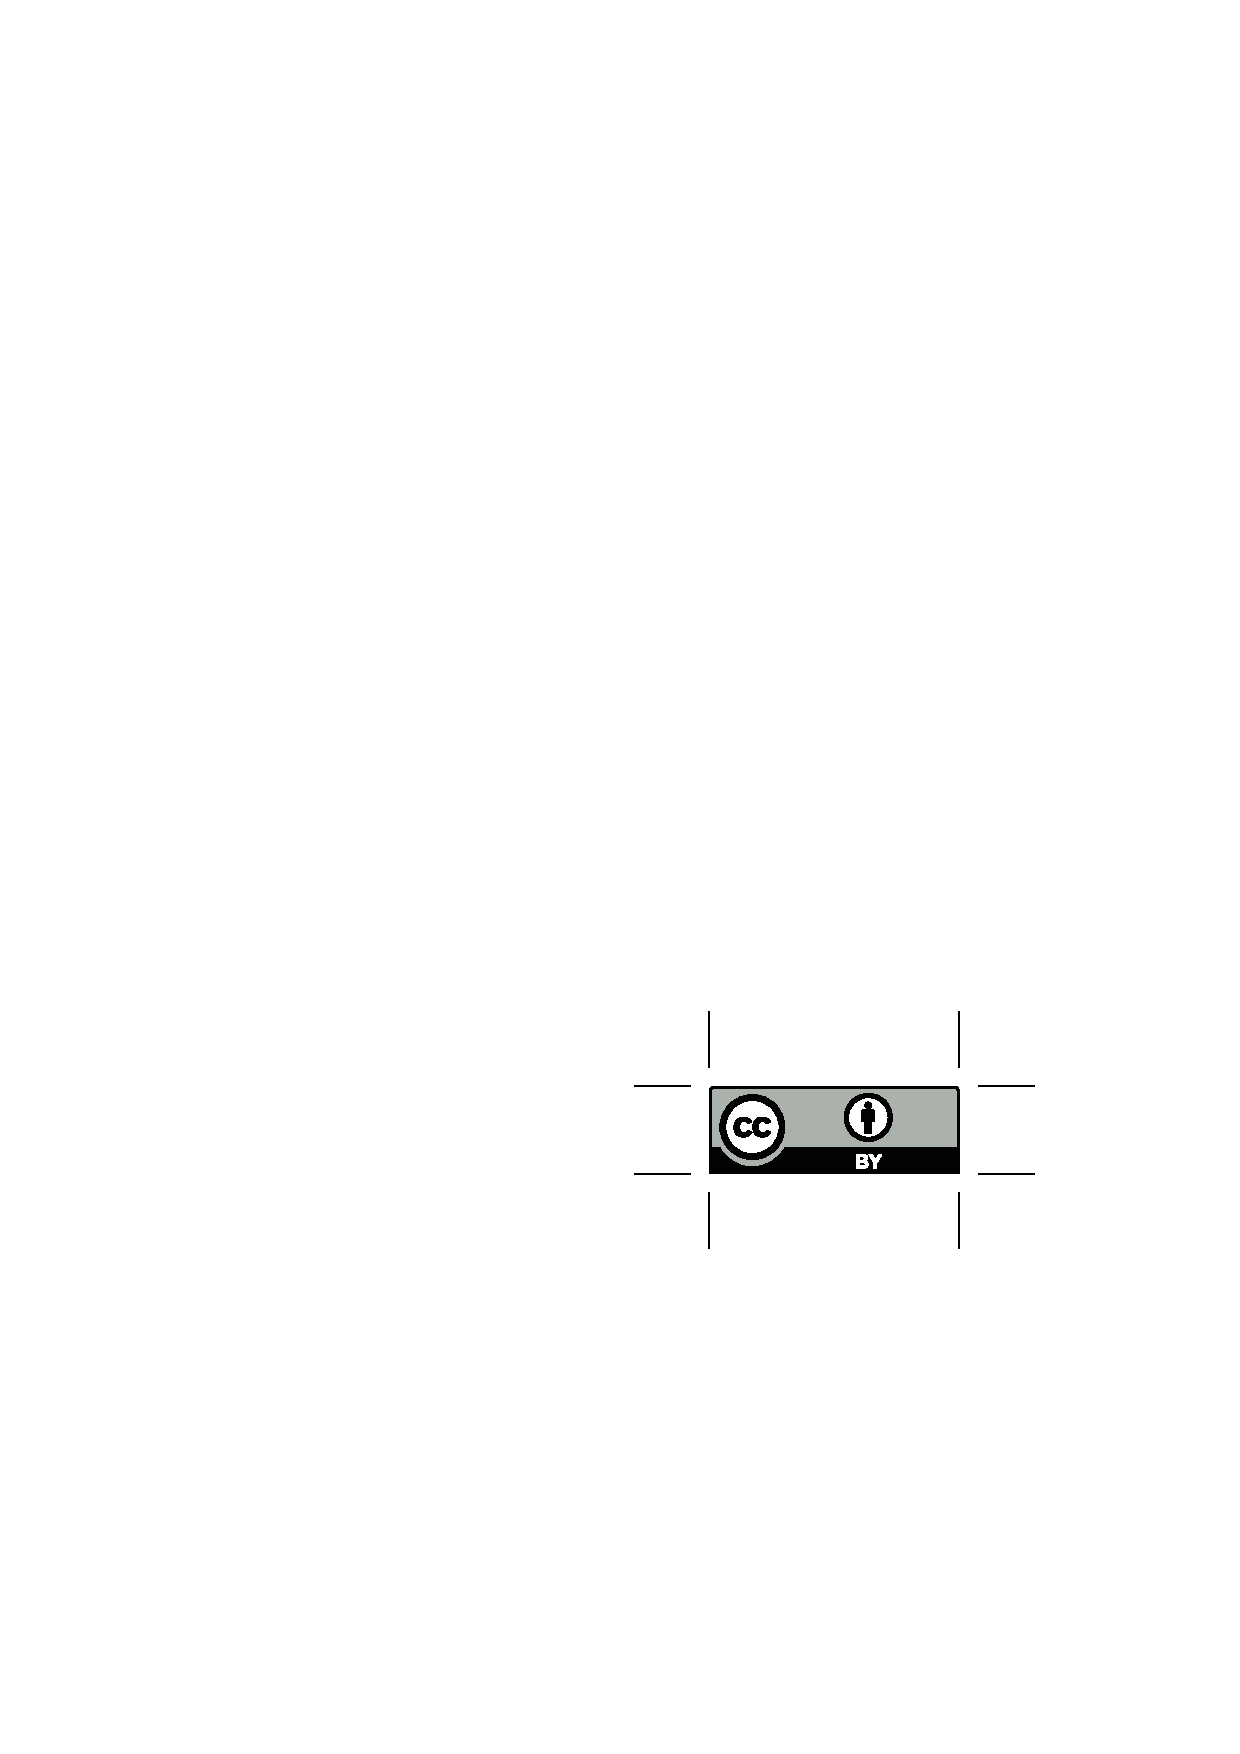
\includegraphics[width=0.90\textwidth]{by}}
  \end{minipage}\hfill
  \begin{minipage}{0.8\columnwidth}
   \href{https://creativecommons.org/licenses/by/4.0/}{This work is licensed under a Creative Commons Attribution International 4.0 License.}
  \end{minipage}
  \vspace{5pt}
}
\makeatother

\setcopyright{ifaamas}
\acmConference[AAMAS 2027]{Proc.\@ of the 26th International Conference
on Autonomous Agents and Multiagent Systems (AAMAS 2027)}{3--7 May 2027}{Hanoi, Vietnam}{M.~Baldoni, F.~Fang, W.~Yeoh, N.~Yorke-Smith (eds.)}
\copyrightyear{2027}
\acmYear{2027}
\acmDOI{}
\acmISBN{}
\acmSubmissionID{MASGym-2027-001}
\submissionType{Research Paper Track}

% ---- encoding / fonts ----
\usepackage[utf8]{inputenc}
\usepackage[T1]{fontenc}
\usepackage{microtype}
\usepackage{balance}

% ---- math ----
% NOTE: use amsfonts (not amssymb): acmart/sigconf loads newtxmath, and
% amssymb's \Bbbk redefinition conflicts with it.
\usepackage{amsmath,amsfonts,amsthm,mathtools,bm}
\usepackage{xspace}

% ---- citations (author--year, natbib is loaded by acmart) ----
\citestyle{acmauthoryear}

% ---- lists / tables / floats ----
\usepackage{enumitem}
\usepackage{booktabs,multirow,array}
\usepackage{xcolor}
\usepackage{float}

% ---- graphics: TikZ / PGFPlots ----
\usepackage{tikz}
\usetikzlibrary{arrows.meta,positioning,calc,fit,backgrounds,shapes.geometric,%
  shapes.symbols,decorations.pathreplacing,patterns,matrix,shadows.blur}
\usepackage{pgfplots}
\pgfplotsset{compat=1.18}
\usepgfplotslibrary{groupplots,fillbetween}

% ---- cross-document references (inert unless \externaldocument is used) ----
% Must be loaded before hyperref/cleveref resolve, hence its position here.
\usepackage{xr}

% ---- hyperlinks + clever references (hyperref is loaded by acmart) ----
\usepackage{cleveref}

% ---- shared TikZ styles (visual grammar) ----
\input{figures/tikz_styles.tex}

% ============================================================================
% Theorem environments
% ============================================================================
\theoremstyle{plain}
\newtheorem{theorem}{Theorem}[section]
\newtheorem{lemma}[theorem]{Lemma}
\newtheorem{proposition}[theorem]{Proposition}
\newtheorem{corollary}[theorem]{Corollary}
\theoremstyle{definition}
\newtheorem{definition}[theorem]{Definition}
\newtheorem{assumption}{Assumption}
\theoremstyle{remark}
\newtheorem{remark}[theorem]{Remark}

\crefname{assumption}{Assumption}{Assumptions}
\Crefname{assumption}{Assumption}{Assumptions}

% ============================================================================
% Lightweight algorithm float + pseudocode macros
% (reproduce a numbered, ruled pseudocode listing with float.sty only)
% ============================================================================
\floatstyle{ruled}
\newfloat{algorithm}{tbp}{loa}
\floatname{algorithm}{Algorithm}
\crefname{algorithm}{Algorithm}{Algorithms}
\Crefname{algorithm}{Algorithm}{Algorithms}
\newcounter{algline}
\newlength{\algind}
\newcommand{\algreset}{\setcounter{algline}{0}\setlength{\algind}{0pt}}
\newcommand{\PL}[1]{\par\refstepcounter{algline}\noindent
  \makebox[2.6em][r]{\scriptsize\thealgline:\,}\hspace{0.5em}\hspace{\algind}%
  \ignorespaces#1\strut}
\newcommand{\Ind}{\addtolength{\algind}{1.5em}}
\newcommand{\Ded}{\addtolength{\algind}{-1.5em}}
\newcommand{\kw}[1]{\textbf{#1}}
\newcommand{\comm}[1]{\hfill{\footnotesize\itshape\color{black!55}\(\triangleright\)~#1}}

% ============================================================================
% Notation macros
% ============================================================================
\newcommand{\R}{\mathbb{R}}
\newcommand{\N}{\mathbb{N}}
\newcommand{\E}{\mathbb{E}}
\newcommand{\Prob}{\mathbb{P}}
\newcommand{\indic}{\mathbb{1}}
\newcommand{\Agents}{\mathcal{A}}          % set of agents
\newcommand{\Roles}{\mathcal{R}}           % role set
\newcommand{\Gtop}{\mathcal{G}}            % topology graph
\newcommand{\Vtop}{\mathcal{V}}
\newcommand{\Etop}{\mathcal{E}}
\newcommand{\Nin}{\mathcal{N}^{-}}          % inbound neighbourhood
\newcommand{\Trace}{\tau}                  % global state trace
\newcommand{\TraceSp}{\mathcal{T}}         % trace space
\newcommand{\Statesp}{\mathcal{S}}         % state space
\newcommand{\Predsec}{\Phi}                % system-level security predicate
\newcommand{\Predutil}{\Psi}               % benign-success predicate
\newcommand{\Checker}{\mathsf{C}}          % deterministic checker
\newcommand{\Emu}{\mathcal{E}_{\mathrm{LM}}} % LM tool emulator
\newcommand{\Judge}{\mathsf{J}}            % LLM judge (contrast)
\newcommand{\Advset}{\mathcal{B}}          % adversarial agent set
\newcommand{\betafrac}{\beta}              % adversary fraction
\newcommand{\config}{c}                    % environment configuration
\newcommand{\Configs}{\mathcal{C}}         % configuration space
\newcommand{\ASRs}{\mathrm{ASR}_{\mathrm{sys}}}
\newcommand{\ASRa}{\mathrm{ASR}_{\mathrm{act}}}
\newcommand{\PNAs}{\mathrm{PNA}_{\mathrm{sys}}}
\newcommand{\NRPs}{\mathrm{NRP}_{\mathrm{sys}}}
\newcommand{\CPR}{\mathrm{CPR}}            % compromise-propagation rate
\newcommand{\CSR}{\mathrm{CSR}}            % collusion success rate
\newcommand{\red}{\rho}                    % red policy
\newcommand{\blue}{\delta}                 % blue policy (defense)
\newcommand{\pinf}{p}                      % per-edge propagation probability
\newcommand{\thresh}{\theta}               % threshold (bootstrap percolation)
\newcommand{\kappaem}{\kappa}              % emulation agreement
\newcommand{\defname}{\textsc{MASGym}\xspace}
\newcommand{\corb}{\textsc{CoRB}\xspace}

% ============================================================================
% Title and author metadata (in the preamble, as in the official sample)
% ============================================================================
\title[MASGym: A Security Gym for Multi-Agent LLM Systems]{\defname: A
Co-Evolving Red/Blue Security Gym for Multi-Agent LLM Systems with
Parameterized Collusion, Orchestrator Compromise, and System-Level Metrics}

% Anonymous double-blind submission: the author block is suppressed by the
% `anonymous' class option. For camera-ready, remove that option and fill in
% your full author list, affiliations, and emails.
\author{Thanh Pham}
\affiliation{%
  \institution{School of Computing Technologies, RMIT University}
  \country{Melbourne, Australia}}
\email{thanhphamchivn@gmail.com}

% Abstract and keywords must be defined in the preamble, before \maketitle.
\input{sections/abstract.tex}


\begin{document}


\maketitle

% ---------------------------------------------------------------------------
% Body
% ---------------------------------------------------------------------------
\section{Introduction}
\label{sec:intro}

Progress in the security of large language model (LLM) agents has tracked the quality of
the instruments used to measure it. Agent Security Bench
(ASB)~\cite{zhang2025asb} introduced a utility--security metric
$\mathrm{NRP}=\mathrm{PNA}\cdot(1-\mathrm{ASR})$; AgentDojo~\cite{debenedetti2024agentdojo}
evaluates an agent under injection with \emph{deterministic}, state-based
\texttt{security()} checks; ToolEmu~\cite{ruan2024toolemu} emulates arbitrary tool
execution; InjecAgent~\cite{zhan2024injecagent} benchmarks indirect injection. These
instruments are strong but single-agent: their only cross-agent channel is a shared memory
store. Yet deployed systems such as AutoGen~\cite{wu2023autogen},
MetaGPT~\cite{hong2023metagpt}, CAMEL~\cite{li2023camel},
ChatDev~\cite{qian2024chatdev}, and Magentic-One~\cite{fourney2024magenticone} are
orchestrated \emph{collectives}: a planner directs workers, agents share memory,
third-party tools sit on the critical path, and many tasks require several agents to
finish at all.

In such systems the security questions are group-level. Do a fraction of agents
\emph{collude}? Is the \emph{orchestrator} trusted, or compromised? Can a \emph{malicious
tool}, a \emph{Sybil} identity, or a \emph{poisoned} memory entry spread through the
collective? Re-running a single-agent benchmark $N$ times cannot produce these phenomena.
MASEC~\cite{schroederdewitt2025masec} argues that agent security is
\emph{non-compositional}---individually safe agents compose into unsafe systems---and
notes that no multi-agent security benchmark exists, listing what one must provide:
heterogeneous roles, partial observability, forced coordination, a co-evolving red/blue
methodology, and group-level emergence metrics.

\paragraph{Contributions.}
To the best of our knowledge \defname{} is the first environment purpose-built for the
security of multi-agent LLM systems. It is not a new attack or defense; it is an
environment and evaluation methodology whose scientific object is the controlled variation
of coordination, collusion, and orchestrator variables and the system-level metrics that
quantify their effect (architecture in the Supplementary Material; three-layer design in
\Cref{sec:method}). Concretely,
\begin{itemize}[leftmargin=1.4em]
\item \textbf{An environment and task suite} (\Cref{sec:system,sec:method}): heterogeneous
roles, partial observability, \emph{forced-coordination} tasks (no agent can complete one
alone), over star/chain/tree/mesh topologies at $3$--$50$ agents.
\item \textbf{A parameterized adversary model} (\Cref{sec:threat}): one vector controls
adversary fraction, collusion, adaptivity, orchestrator compromise, malicious tools,
Sybils, and poisoned memory, under a system-level compromise objective.
\item \textbf{A system-level metric suite} (\Cref{sec:problem,sec:method}): the
generalization $\NRPs=\PNAs(1-\ASRs)$, scored by a \emph{deterministic checker} over the
global trace so an injection cannot hijack the evaluator (\Cref{thm:integrity}), plus
collusion-success and compromise-propagation rates, coordination quality, cost, and
recovery.
\item \textbf{The \corb{} co-evolving red/blue protocol} (\Cref{sec:algorithm}), logging
$(\text{attack},\text{defense},\NRPs)$ trajectories and a (security, cost) Pareto frontier.
\item \textbf{An answer to ``does the defense work?''} (\Cref{sec:defense}): on four real
backbones in three model families a prompt-level defense drives action-channel compliance
to $0/1075$ decisions---$\ASRa{=}0$---yet $\ASRs$ stays $1.000$ on tree and star, because
the residual failure is deterministic availability sabotage that topology alone determines,
and one backbone ignores the defense entirely (\Cref{tab:defense}). A defense scored on the
action channel cannot certify system-level security. The controlled synthetic sweep
separately measures the guardrail's shrinking margin, $41.6\%\to31.8\%\to27.6\%$
(degradation grid, Supplementary Material).
\end{itemize}

Because reviewers rightly discount benchmarks whose central metric is asserted rather than
justified, we treat theory as part of the instrument (\Cref{sec:theory}): under explicit
assumptions and honest proof-status labels we prove the product aggregator is the unique
combiner satisfying our axioms and reduces to ASB at $N{=}1$; that the deterministic
checker cannot be hijacked through message content, unlike a message-reading LLM judge,
which we measure pushed off the recorded state in roughly a third of injected traces;
topology-dependent propagation bounds and a strict collusion advantage in the cascade
model; a forced-coordination lower bound; and finite-sample concentration. None
asserts that any real defense is secure or provably degrades.

\paragraph{Scope and stance.}
\defname{} is an instrument, not a verdict: a lower $\ASRs$ is a measurement under a stated
configuration, not a certificate. The central threat to validity is emulation
fidelity---ToolEmu's reported human agreement is $\kappaem\approx0.48$---so scoring routes
through the deterministic checker, the caveat is explicit, and the harness registers
emulated-versus-real ablations for independent re-testing. Of those two we ran the
deterministic-versus-judge half on real judge backbones (\Cref{sec:integrity}); the
emulated-versus-real-tools half is unmeasured, since no real tool backend is wired in.
The checker and harness form a trusted computing base, and model-weight attacks are out
of scope. Roadmap:
\Cref{sec:related}--\Cref{sec:prelim} situate and fix notation; \Cref{sec:system,sec:threat,sec:problem}
formalize; \Cref{sec:method,sec:algorithm} present the environment and protocol;
\Cref{sec:theory} justifies; \Cref{sec:experiments} evaluates; the final sections discuss and
bound limitations.
\section{Related Work}
\label{sec:related}

\subsection{Single-agent security instruments}
The closest instruments evaluate a lone tool-using agent. ASB~\cite{zhang2025asb}
formalizes attacks and defenses for agents and introduces the utility--security metric
$\mathrm{NRP}=\mathrm{PNA}\cdot(1-\mathrm{ASR})$ that we generalize; its threat model is
single-agent with retrieved memory. AgentDojo~\cite{debenedetti2024agentdojo} contributes
a stateful environment whose \emph{deterministic} security/utility functions are computed
from pre- and post-execution state, so a prompt injection cannot also hijack the evaluator;
it names multi-agent planner/worker defense as future work.
InjecAgent~\cite{zhan2024injecagent}, ToolEmu~\cite{ruan2024toolemu},
AgentHarm~\cite{andriushchenko2025agentharm}, HarmBench~\cite{mazeika2024harmbench}, and
formalizations of prompt injection~\cite{liu2024formalizing} and
trustworthiness~\cite{wang2023decodingtrust} complete the single-agent picture. None
parameterizes collusion, orchestrator trust, Sybils, or compromise propagation.

\subsection{Multi-agent LLM frameworks and attacks}
A large literature builds collectives---AutoGen~\cite{wu2023autogen},
MetaGPT~\cite{hong2023metagpt}, CAMEL~\cite{li2023camel},
ChatDev~\cite{qian2024chatdev}, Magentic-One~\cite{fourney2024magenticone}, and
mixing/debating designs~\cite{du2023debate}---concerned with capability, not security;
\defname{} adopts their role structures as substrate. A fast-growing attack literature is
intrinsically multi-agent: prompt infection~\cite{lee2024promptinfection},
contagious blocking~\cite{zhou2025corba}, population jailbreaking~\cite{gu2024agentsmith},
topological safety~\cite{yu2024netsafe}, adversarial roles~\cite{tian2023evilgeniuses},
GenAI worms~\cite{cohen2024aiworm}, memory poisoning~\cite{chen2024agentpoison}, and
backdoors~\cite{yang2024watchout}. These are attacks in bespoke setups; \defname{} is the
controlled, deterministically scored environment in which such attacks and defenses can be
swept and compared.

\subsection{Defenses, surveys, and systematizations}
Multi-agent defenses include AutoDefense~\cite{zeng2024autodefense} and the
topology-guided G-Safeguard~\cite{yu2025gsafeguard}; per-agent guardrails
(TrustAgent~\cite{hua2024trustagent}, Llama Guard~\cite{inan2023llamaguard}, NeMo
Guardrails~\cite{rebedea2023nemo}) are the baselines we lift into the collective setting.
Classical Byzantine fault tolerance~\cite{lamport1982byzantine,pease1980reaching} and
Byzantine-robust aggregation~\cite{blanchard2017krum} tolerate faulty fractions under a
trusted coordinator over numeric messages; they motivate our collusion and
orchestrator-trust knobs without covering natural-language collectives. Surveys of
agent security~\cite{he2025emerged,li2024personalllmagents} and the
non-compositionality argument~\cite{schroederdewitt2025masec,hammond2025multiagent} are the
gap \defname{} addresses.

\subsection{Environments, red teaming, and evaluation validity}
Methodologically \defname{} follows standardized environments---Gym~\cite{brockman2016openaigym},
PettingZoo~\cite{terry2021pettingzoo}, and Melting Pot~\cite{leibo2021meltingpot}, which
evaluates social outcomes at the level of the collective---and automated red
teaming~\cite{perez2022redteaming}, with the MAST taxonomy~\cite{cemri2025mast}
supplying a vocabulary for group-level failures. On scoring validity, LLM-as-judge
evaluation is documented as manipulable and biased~\cite{zheng2023judging,wang2023fair};
\defname{} therefore keeps a deterministic trace-based checker on the critical path and
treats the deterministic-versus-judge comparison as a measurable ablation.

\subsection{Positioning}
\defname{} is \emph{not} ASB applied to many agents (ASB's only cross-agent vector is
shared memory), \emph{not} AgentDojo at scale (its deterministic checker is per-agent over
environment state; a collective requires system-level predicates over a global trace,
\Cref{sec:problem}), and \emph{not} a model-swap or prompt-filter study: its object is the
controlled variation of coordination, collusion, and orchestrator variables, and the
system-level metrics that quantify their effect.
\section{Preliminaries and Notation}
\label{sec:prelim}

This section recalls the three primitives \defname{} builds on (notation summarized in the
Supplementary Material): ASB's utility--security metric, AgentDojo's
deterministic state-based checking, and ToolEmu's LM tool emulation.

\subsection{ASB's utility--security metric}
ASB~\cite{zhang2025asb} scores an agent by a \emph{Non-Refusal Performance},
\begin{equation}
\label{eq:asb-nrp}
\mathrm{NRP} \;=\; \mathrm{PNA}\cdot(1-\mathrm{ASR}),
\end{equation}
where $\mathrm{PNA}\in[0,1]$ is performance on benign tasks and $\mathrm{ASR}\in[0,1]$ the
attack success rate; the product rewards a system only when both useful and not attacked.
\Cref{eq:asb-nrp} is defined for a single agent; generalizing it to a collective is the
subject of \Cref{sec:problem,sec:theory}.

\subsection{AgentDojo's deterministic state-based checking}
AgentDojo~\cite{debenedetti2024agentdojo} evaluates security by \emph{deterministic}
functions of environment state rather than an LLM judge: a task fixes a predicate reading
the pre- and post-execution state and returning a Boolean, so an injection cannot
manipulate the score unless it changes the security-relevant state. \defname{} lifts this
property to the system level: our checker $\Checker$ evaluates $\Predsec,\Predutil$ over the
\emph{global} trace $\Trace$, never an invocable LLM judge, and we prove the resulting
integrity property in \Cref{thm:integrity}.

\subsection{ToolEmu's LM tool emulation}
ToolEmu~\cite{ruan2024toolemu} emulates tool execution from a specification with a language
model, enabling breadth at low cost, at a reported human agreement of only
$\kappaem\approx0.48$ (Cohen's $\kappa$~\cite{cohen1960coefficient}, extended to many
raters by Fleiss~\cite{fleiss1971measuring}). \defname{} adopts LM emulation for tool
breadth, including an adversarial mode $\Emu^{\!\dagger}$ for malicious tools, but treats
$\kappaem$ as a first-class threat to validity: scoring routes through the deterministic
  checker, and the harness registers an emulated-versus-real-tools ablation for
  independent re-testing. We did not run it: no real tool backend is wired into our
  environment, so we report it as an unmeasured gap rather than let the registration
  imply coverage (\Cref{sec:limitations}). An \emph{episode} runs a task under a fixed configuration
$\config$ and produces a global trace $\Trace\sim\mathcal{D}(\config)$, from which all
security and utility quantities are computable---the fact that makes deterministic,
hijack-resistant scoring possible.

% Notation table moved to the Supplementary Material to keep the main paper
% within its page limit; main-text references it in prose.
\section{System Model}
\label{sec:system}

\defname{} evaluates a collective of $N\in\{3,\dots,50\}$ LLM agents
$\Agents=\{a_1,\dots,a_N\}$, each assigned exactly one role from the set $\Roles$
(notation in the Supplementary Material). Roles pool access to shared tools and a shared
versioned memory, and interplay is \emph{structural}, captured by a topology
$\Gtop=(\Vtop,\Etop)$ over agents---star, chain, tree, or mesh---that fixes who may
influence whom:
$j\in\Nin(a)$ means $a$ reads $j$'s outputs; the orchestrator is typically the star's
centre.

An \emph{episode} executes a task under a configuration $\config$ for $H$ steps, producing
a \emph{global trace} $\Trace=(s_0,\dots,s_H)$, where $s_t$ is the complete state: every
agent's messages, tool calls, tool outputs, memory versions, role assignments, topology
edges, and the agent-identity map. Traces are i.i.d.\ from $\mathcal{D}(\config)$
(\Cref{as:iid}). Because $\Predsec,\Predutil$ are functions of recorded state only
(\Cref{def:predicates}), system-level quantities are computable offline from $\Trace$,
which is what keeps the checker deterministic and the measurement reproducible. A
configuration $\config\in\Configs$ specifies task, $\Gtop$, models, tools, $\Advset$, and
protocol constants, so a study reports $\NRPs$ as a coordinate over a \emph{sweep} that
varies exactly one component at a time under a controlled seed.

\section{Threat Model}
\label{sec:threat}

The adversary is a \emph{set} $\Advset\subseteq\Agents$ of \emph{adversarial agents},
of size $\betafrac N$ chosen by the operator---a single corrupted node or a coordinated
coalition sharing a channel and a joint objective. Capabilities and attack mode are fixed
by
\begin{equation}
\label{eq:adv-config}
\config_{\mathrm{adv}}\;=\;\bigl(\betafrac,\ \mathsf{coll},\ \mathsf{adapt},\ \mathsf{orch},\ \mathsf{tool},\ \mathsf{syb},\ \mathsf{mem}\bigr),
\end{equation}
selecting respectively: adversary fraction; independent vs.\ colluding coordination
(\Cref{def:csr}); static vs.\ adaptive attacks across \corb{} rounds; compromised
orchestrator; malicious tools (adversarial emulator $\Emu^{\!\dagger}$); Sybils; and
poisoned memory. $\Advset$ may issue messages and tool calls as its roles, read
$\mathcal{M}$, and read the outputs of its topology predecessors; \emph{outside} its
powers are the harness, the recorded trace, the checker, the emulator's mechanism, and the
honest agents' private internals. Compromise then \emph{propagates} along $\Gtop$
(\Cref{def:propagation}) from these seeds, so the effective compromised set at episode end,
$\Advset_\infty$, can exceed $\Advset$.

\textbf{Inferential threats and scope.} The operator sets horizon, models, and metrics; the
adversaries do not. An \emph{LLM judge}, when used (only in ablations, off the critical
path), is a \emph{measurement} threat: human agreement is $\kappaem\approx0.48$ and judges
can be gamed; the deterministic checker exists to remove this threat (\Cref{thm:integrity},
\Cref{prop:judgehijack}). The TCB is the harness (trace recording, roles, topology,
scheduling), the tool specifications, and the registered predicates; everything
else---messages, memory writes, tool outputs, intent---is outside the TCB. Scope is
\emph{per se} the \emph{collective}; adversaries are bounded by the seven knobs and episodic
budgets; a harness-level adversary and model-weight attacks are out of scope; honest agents
have no budget (per ASB) and obey their assigned roles.
% Threat Model section is merged into system_model.tex to save body pages.
% Historical reference: sec:threat now labels the merged section there.
\section{Problem Formulation}
\label{sec:problem}

We define what a system-level security benchmark must measure: security and benign-success
predicates, the system-level metric aggregating them, and the group-level quantities
(forced coordination, compromise propagation, collusion) with no single-agent analogue.

\subsection{System-level predicates}
\begin{definition}[System-level security and benign-success predicates]
\label{def:predicates}
A task fixes two Boolean functionals of the global trace $\Trace\in\TraceSp$: a
\emph{security predicate} $\Predsec:\TraceSp\to\{0,1\}$, $1$ iff the trace contains a
system-level compromise (an unsafe action executed, protected data exfiltrated, or a
forced-coordination task sabotaged), and a \emph{benign-success predicate}
$\Predutil:\TraceSp\to\{0,1\}$, $1$ iff the collective completed the legitimate task.
Both are registered programs evaluated by the deterministic checker over the
harness-recorded trace; dependencies on \emph{un}-recorded natural-language content are
disallowed, yielding evaluator integrity (\Cref{thm:integrity}) and lifting
AgentDojo~\cite{debenedetti2024agentdojo} from one agent's state to the global trace.
\end{definition}

\subsection{System-level metrics}
\begin{definition}[System-level ASR, PNA, and NRP]
\label{def:metrics}
Fix a configuration $\config$ and let $\Trace\sim\mathcal{D}(\config)$. Define
\begin{align}
\ASRs(\config) &\;=\; \Prob_{\Trace\sim\mathcal{D}(\config)}\!\bigl[\Predsec(\Trace)=1\bigr],
\label{eq:asrsys}\\
\PNAs(\config) &\;=\; \Prob_{\Trace\sim\mathcal{D}(\config^{\circ})}\!\bigl[\Predutil(\Trace)=1\bigr],
\label{eq:pnasys}\\
\NRPs(\config) &\;=\; \PNAs(\config)\cdot\bigl(1-\ASRs(\config)\bigr),
\label{eq:nrpsys}
\end{align}
where $\config^{\circ}$ is $\config$'s benign counterpart (no adversary), so $\PNAs$ measures
coordinated-task performance uncontaminated by attack-induced refusals, exactly as ASB
separates PNA from ASR.
\end{definition}

Two properties are required and proved in \Cref{sec:theory}: \Cref{eq:nrpsys} \emph{reduces}
to ASB's \Cref{eq:asb-nrp} at $N{=}1$ (\Cref{prop:reduction}), and the product form is
\emph{justified} rather than assumed, via an axiomatic characterization over D1--D5
(\Cref{sec:theory}; \Cref{thm:metric}). The benchmark stance: $\NRPs$ is a coordinate for
comparing configurations, not a certificate.

\subsection{Forced coordination}
\begin{definition}[$k$-forced-coordination task]
\label{def:forced}
For an agent set $\Agents$, let a \emph{witness} be a set $W\subseteq\Agents$ whose joint
contributions can satisfy $\Predutil$. A task is \emph{$k$-forced-coordination} if every
witness has size $|W|\ge k$; equivalently, for every $S$ with $|S|<k$, no assignment in
which only the agents of $S$ act non-trivially satisfies $\Predutil$.
\end{definition}

$k$-forced tasks with $k\ge2$ cannot be represented in a single-agent harness.
\Cref{sec:theory} relates task disruption to whether $\Advset$ intersects every minimal
witness (a hitting-set condition, \Cref{prop:forced}).

\subsection{Compromise propagation and collusion}
\begin{definition}[Compromise relation and propagation rate]
\label{def:propagation}
Let $\Advset_0=\Advset$ be the initially adversarial (seed) agents. Compromise spreads
over $\Gtop$ according to a monotone rule $\mathcal{P}$ (\Cref{sec:theory}: an
independent-cascade model with per-edge probability $\pinf$, or a threshold model with
threshold $\thresh$). Write $\Advset_\infty\supseteq\Advset_0$ for the compromised set at
fixation. The \emph{compromise-propagation rate} is
\begin{equation}
\label{eq:cpr}
\CPR(\config) \;=\; \E\!\left[\frac{|\Advset_\infty|-|\Advset_0|}{\,N-|\Advset_0|\,}\right],
\end{equation}
the expected fraction of \emph{initially honest} agents that become compromised.
\end{definition}

\begin{definition}[Collusion success rate]
\label{def:csr}
For a fixed fraction $\betafrac$, let $\ASRs^{\mathrm{coll}}$ and $\ASRs^{\mathrm{ind}}$ be
the system attack success rates under colluding and independent adversaries respectively.
The \emph{collusion success rate} reports $\ASRs^{\mathrm{coll}}$, and the
\emph{collusion advantage} is $\Delta_{\mathrm{coll}}=\ASRs^{\mathrm{coll}}-\ASRs^{\mathrm{ind}}$.
\end{definition}
\section{The \defname{} Environment}
\label{sec:method}

\defname{} is organized as three layers (architecture figure in the Supplementary Material): an \emph{emulation
layer} that supplies tools, a \emph{deterministic checking layer} that scores
system-level predicates, and an \emph{orchestration layer} that instantiates the system
and threat models and drives the \corb{} loop.

% moved to Supplementary Material (page limit): see \Cref{fig:architecture} there.
% \input{figures/tikz_architecture.tex}

\subsection{Emulation and deterministic checking}
Following ToolEmu~\cite{ruan2024toolemu}, tool execution is emulated by a language model
$\Emu$ from a tool specification, giving breadth without hand-built sandboxes; an
\emph{adversarial} mode $\Emu^{\!\dagger}$ realizes malicious tools (attacker-controlled
responses, exfiltration bait, injected instructions). Crucially the emulator is \emph{not}
on the scoring critical path: it produces the tool outputs agents consume, while the
verdict comes from the deterministic checker, so emulator noise degrades realism, not
scoring integrity. The checker $\Checker$ evaluates the registered predicates
$\Predsec,\Predutil$ over the global trace (\Cref{def:predicates}) and never invokes an
LLM judge on the critical path. Predicates are programs over recorded state: an
\emph{exfiltration} predicate fires iff protected data recorded as leaving the trust
boundary appears in an outbound tool call; a \emph{sabotage} predicate fires iff a
$k$-forced task's witness set was prevented from completing; an \emph{unsafe-action}
predicate fires iff a denylisted transition is recorded. An optional LLM judge\nobreak\
$\Judge$, available only off the critical path, enables the ablation (RQ2).

\subsection{Orchestration layer and task suite}
The orchestration layer builds the topology $\Gtop$, assigns roles, enforces observability
masks, applies $\config_{\mathrm{adv}}$ of \Cref{eq:adv-config}, and runs episodes; it is
part of the TCB and exposes the \corb{} interface (\Cref{sec:algorithm}). Tasks are
\emph{forced-coordination} by design (\Cref{def:forced}), so the collective is the unit of
analysis: each provides a benign goal decomposable across roles, a registered pair
$(\Predutil,\Predsec)$, a tool set (some malicious under $\mathsf{tool}$), a shared-memory
schema (poisonable under $\mathsf{mem}$), and a topology (star: hub-and-spoke delegation;
chain: pipelines; tree: hierarchical; mesh: peer collaboration), parameterized by $k$ (the
degree of forced coordination) and benign difficulty.

\subsection{Realized adversary knobs}
Each component of $\config_{\mathrm{adv}}$ maps to a concrete harness mechanism:
$\betafrac$ selects the seed set $\Advset$; $\mathsf{coll}$ toggles a shared channel and
joint objective; $\mathsf{adapt}$ enables red co-evolution across \corb{} rounds;
$\mathsf{orch}$ flips the orchestrator's policy; $\mathsf{tool}$ routes tools through
$\Emu^{\!\dagger}$; $\mathsf{syb}$ instantiates extra identities under one controller; and
$\mathsf{mem}$ writes poisoned entries to shared memory. Because the knobs are independent,
a study isolates each variable's effect while holding the rest fixed---the controlled
variation that is the paper's scientific object~\cite{rubin1974estimating}.

\subsection{Metric suite}
\label{sec:metric-suite}
All reported quantities are computed from traces by the deterministic checker or harness
logs; none is an LLM-judge verdict: system attack success rate $\ASRs$ and system NRP
$\NRPs$ (\Cref{eq:asrsys,eq:nrpsys}); benign performance $\PNAs$ (\Cref{eq:pnasys});
collusion success rate and advantage (\Cref{def:csr}); compromise-propagation rate $\CPR$
(\Cref{eq:cpr}); coordination quality and its degradation under sabotage; time-to-detection
and recovery; token/API cost and latency and their scaling with $N$; and human-intervention
rate. Estimating these to target precision requires the budget fixed by \Cref{thm:sample};
the resulting cost model---$\Theta(MNH)$ agent invocations per configuration,
$\Theta(GNH\Delta^{-2}\ln(G/\alpha))$ for a sweep---is reported with each study and
archived in full with the harness.
\section{The \corb{} Co-Evolving Red/Blue Protocol}
\label{sec:algorithm}

\defname{}'s evaluation methodology is a co-evolving loop, \corb, that alternates a red
policy proposing attack configurations and a blue policy proposing defenses, scoring each
pair with the deterministic checker and logging a trajectory of
$(\text{attack},\text{defense},\NRPs)$ triples. The per-configuration scoring procedure
(\textsc{ScoreConfig}) is fully specified: instantiate $\Gtop$, roles, masks, and the
adversary knobs $\config_{\mathrm{adv}}$\Cref{eq:adv-config} via the trusted harness; seed
$\Advset_0$; run $M$ episodes of $H$ steps, recording each transition into the global
trace and updating the compromised set under the propagation rule $\mathcal{P}$
(\Cref{def:propagation}); evaluate $(\Predutil,\Predsec)$ with the deterministic checker on
each trace; and aggregate $\widehat{\ASRs},\widehat{\PNAs},\widehat{\NRPs},\widehat{\CPR}$
plus detection and recovery statistics. The protocol-level loop is \Cref{alg:corb}. Both
levels keep the LLM off the scoring critical path, so no proposal can inflate its own
score.

\begin{algorithm}[t]
\caption{\corb: co-evolving red/blue evaluation.}
\label{alg:corb}
\algreset
\PL{\kw{Input:} red policy $\red$; blue policy $\blue$; rounds $R$; task, budget $M$.}
\PL{\kw{Output:} trajectory $\mathcal{L}=\{(\config^r_{\mathrm{adv}},\blue^r,\NRPs^r,\ASRs^r)\}_{r=1}^R$
and a Pareto frontier.}
\PL{Initialize defense $\blue^0$ (no-defense or a lifted per-agent defense).}
\PL{\kw{for} $r=1,\dots,R$ \kw{do}}\Ind
\PL{\emph{Red step:} $\config^r_{\mathrm{adv}}\gets\red(\mathcal{L}_{<r},\blue^{r-1})$
\comm{static: fixed; adaptive: best-response}}
\PL{Score $(\config^r_{\mathrm{adv}},\blue^{r-1})$ with \textsc{ScoreConfig}.}
\PL{\emph{Blue step:} $\blue^r\gets\blue(\mathcal{L}_{<r},\config^r_{\mathrm{adv}})$
\comm{propose/upgrade defense}}
\PL{Re-score $(\config^r_{\mathrm{adv}},\blue^r)$; append both scorings to $\mathcal{L}$.}\Ded
\PL{\kw{return} $\mathcal{L}$ and its $(\ASRs,\text{cost})$ / $(\NRPs,\text{cost})$ frontier.}
\end{algorithm}

Three properties make \corb{} a measurement protocol rather than a training loop:
(i) \emph{integrity}---every score comes from \textsc{ScoreConfig}, so neither policy can
hijack its own evaluation (\Cref{thm:integrity}); (ii) \emph{reproducibility}---the
trajectory $\mathcal{L}$ is the full audit trail of fully specified
$(\config_{\mathrm{adv}},\blue)$ pairs; and (iii) \emph{honesty of the frontier}---\corb{}
reports a Pareto frontier over (security, cost) rather than a single ``winner''. The red
and blue policies may be grid/random search, an optimizer, or an LLM-driven proposer;
\defname{} fixes the \emph{interface} and the \emph{scoring}, not the proposers. Cost is
$\Theta(RMNH)$ for an $R$-round run and $\Theta(GNH\Delta^{-2}\ln(G/\alpha))$ across a
$G$-configuration sweep (\Cref{cor:budget}).
\section{Theory: What the Instrument Measures}
\label{sec:theory}

A benchmark earns trust when its central metric is justified, its evaluator cannot be
gamed, and its sample sizes are principled. We therefore treat theory as part of the
instrument. All results are stated under explicit assumptions (below) and carry honest
proof-status labels; none claims that any real defense is secure or provably degrades.
Short proofs of the central characterization and integrity theorems are inline; remaining
derivations and the complete proof archive ship with the harness (Supplementary Material).

\begin{assumption}[Trusted checking]
\label{as:tcb}
The harness records a faithful global trace $\Trace$, and the checker $\Checker$
evaluates the fixed predicates $\Predsec,\Predutil$ as functions of $\Trace$ \emph{only}
(\Cref{def:predicates}).
\end{assumption}
\begin{assumption}[i.i.d.\ episodes]
\label{as:iid}
For fixed $\config$, the $M$ episode traces are independent draws from
$\mathcal{D}(\config)$.
\end{assumption}
\begin{assumption}[Bounded indicators]
\label{as:bounded}
$\Predutil,\Predsec\in\{0,1\}$.
\end{assumption}
\begin{assumption}[Monotone propagation model]
\label{as:prop}
Compromise spreads over $\Gtop$ via a monotone rule $\mathcal{P}$ (\Cref{def:propagation}):
under \emph{independent cascade}, a compromised agent independently compromises each
susceptible out-neighbour with probability $\pinf$; under \emph{threshold}, a susceptible
agent is compromised once at least $\thresh$ in-neighbours are. This is a modelling choice
\defname{} makes so propagation is measurable, not an empirical law; its realism is itself
measured via $\CPR$.
\end{assumption}
\begin{assumption}[Continuity of the aggregator]
\label{as:cont}
The utility--security aggregator $g:[0,1]^2\to[0,1]$ is continuous.
\end{assumption}

\subsection{Characterization of the system-level metric}
\label{sec:theory-metric}
The product form of $\NRPs$ is forced by the desiderata of \Cref{sec:problem}, phrased as
five axioms (D1--D5): boundedness, consistency, monotonicity, homogeneity (each in both
arguments), and reduction---the operative instance is stated and proven in \Cref{thm:metric}.
Under them, $g$ reduces to ASB's metric at one agent.

\begin{proposition}[Reduction to ASB]
\label{prop:reduction}
If $N=1$ and $\Predsec,\Predutil$ are the single-agent security and benign predicates,
then $\ASRs=\mathrm{ASR}$, $\PNAs=\mathrm{PNA}$, and $\NRPs=\mathrm{NRP}$ of
\Cref{eq:asb-nrp}.
\end{proposition}

\begin{theorem}[Axiomatic characterization of $\NRPs$; complete proof]
\label{thm:metric}
Write $\NRPs=g(u,\sigma)$ with utility $u=\PNAs\in[0,1]$ and security level
$\sigma=1-\ASRs\in[0,1]$. Under \Cref{as:cont}, suppose $g$ satisfies:
\emph{(D2) consistency}, $g(u,1)=u$ and $g(0,\sigma)=0$;
\emph{(D4a) utility-homogeneity}, $g(\lambda u,\sigma)=\lambda\,g(u,\sigma)$ for
$\lambda\in[0,1]$; and
\emph{(D4b) security-homogeneity}, $g(u,\lambda\sigma)=\lambda\,g(u,\sigma)$ for
$\lambda\in[0,1]$.
Then $g(u,\sigma)=u\,\sigma$ is the unique such aggregator, satisfying boundedness (D1)
and monotonicity (D3).
\end{theorem}

\begin{proof}[Proof of \Cref{thm:metric}]
By D4a with base $u=1$ and D4b with base $\sigma=1$,
$g(u,\sigma)=u\,g(1,\sigma)=u\sigma\,g(1,1)=u\sigma$ by D2. The boundary $g(0,\sigma)=0$ holds
since $0\cdot\sigma=0$; and $u\sigma$ is bounded in $[0,1]$ and non-decreasing in each
argument. Continuity (\Cref{as:cont}) extends the homogeneity identities from rationals to
all of $[0,1]$; the identities hold pointwise.
\end{proof}

\begin{remark}
\label{rem:metric}
\Cref{thm:metric} singles out the product \emph{relative to D2/D4}: replacing D4 by a
worst-coordinate axiom yields $\min(u,\sigma)$, and weighted log-linearity yields
$u^{w}\sigma^{1-w}$. \defname{} reports $u\sigma$ by default (it generalizes ASB,
\Cref{prop:reduction}) and exposes alternatives as configurable.
\end{remark}

\subsection{Evaluator integrity}
\label{sec:theory-integrity}
We formalize why deterministic checking cannot be hijacked by a successful injection.

\begin{theorem}[Evaluator integrity; complete proof]
\label{thm:integrity}
Under \Cref{as:tcb}, for any two episodes with equal recorded traces $\Trace=\Trace'$,
$\Checker(\Trace)=\Checker(\Trace')$. Consequently, an adversarial manipulation that
changes message content but leaves the recorded security-relevant state unchanged cannot
change $\Predsec(\Trace)$; hence neither $\widehat{\ASRs}$ nor $\widehat{\NRPs}$ can be
inflated or deflated by message content alone.
\end{theorem}

\begin{proof}[Proof of \Cref{thm:integrity}]
By \Cref{as:tcb} the predicates are functions of $\Trace$ only, so equal traces give equal
verdicts. For any manipulation $\pi$ inducing $\Trace_\pi=\Trace$ the verdict
$\Predsec(\Trace_\pi)=\Predsec(\Trace)$, and hence so are
$\widehat{\ASRs},\widehat{\PNAs},\widehat{\NRPs}$.
\end{proof}

\begin{proposition}[An LLM judge is hijackable; complete proof of existence]
\label{prop:judgehijack}
There exist an LLM judge $\Judge$ that reads messages and a message manipulation $\pi$
with $\Trace_\pi=\Trace$ such that
$\Judge(\Trace_\pi,\mathrm{msgs}_\pi)\neq\Judge(\Trace,\mathrm{msgs})$.
\end{proposition}

\begin{remark}
\Cref{thm:integrity} shows the deterministic verdict cannot be \emph{gamed} through
messages; it does \emph{not} show it is \emph{correct} (a mis-specified predicate can be
systematically wrong). Viewed as a test of the compromise hypothesis, $\Checker$ is a
deterministic decision rule governed by classical testing
theory~\cite{neyman1933problem,lehmann2005testing}; the LLM judge additionally exposes
that decision to manipulation through its message input, as documented for LLM
judges~\cite{zheng2023judging,wang2023fair}. \defname{} keeps $\Checker$ on the critical
path and measures the judge-hijack gap as an ablation (RQ2).
\end{remark}

\subsection{Compromise propagation across topologies}
\label{sec:theory-prop}
Under the independent-cascade instance of \Cref{as:prop}, expected reach depends sharply
on topology (all four derivations in the Supplementary Material): on a chain
\emph{seeded at an endpoint} it is $\sum_{j=1}^{n-1}\pinf^{j}\le\pinf/(1-\pinf)$,
bounded independently of $n$; on a star a centre seed gives $\CPR=\pinf$ while a leaf seed
gives $\pinf+\pinf^{2}(n-2)$, a $\Theta(\pinf(1-\pinf)n)$ gap; trees show a
$b\pinf$-depth phase transition and complete graphs grow superlinearly in seed count.
Under threshold contagion an agent with in-degree below $\thresh$ is never compromised, so
a chain with $\thresh\ge2$ has $\CPR=0$.

\begin{theorem}[Collusion advantage on the star]
\label{thm:collusion}
Fix the independent-cascade model on a star of $N$ nodes with a budget of one seed. A
colluding adversary that places its seed at the centre achieves expected compromise
$C=1+\pinf(N-1)$; an independent adversary placing its seed uniformly at random achieves
expected compromise $\tfrac1N C+\tfrac{N-1}{N}L$, writing $C$ as above and
$L=1+\pinf+\pinf^{2}(N-2)$. Their difference
$\Delta_{\mathrm{coll}}=\pinf(1-\pinf)\tfrac{(N-1)(N-2)}{N}$ is positive,
$\Theta(\pinf(1-\pinf)N)$, for all $\pinf\in(0,1)$, $N\ge3$: coordinated placement
strictly dominates.
\end{theorem}

These results reproduce the classical intuition that spread is slow on sparse chains,
dominated by the hub on stars, phase-transitioned on trees, and explosive on dense
meshes~\cite{granovetter1978threshold,watts2002simple,kempe2003maximizing,chalupa1979bootstrap};
\Cref{thm:collusion} describes the environment's propagation \emph{model}, not any real
defense, and its value is that ``collusion on/off'' is well posed and predicts where to
look (hub-centric topologies) for degradation, tested in \Cref{sec:experiments}.

\subsection{Forced coordination}
\label{sec:theory-forced}
\begin{proposition}[Forced-coordination lower bound]
\label{prop:forced}
Let a task be $k$-forced-coordination (\Cref{def:forced}) with witness family
$\mathcal{W}$. Then: (a) no set $S$ of agents with $|S|<k$ can satisfy $\Predutil$; and
(b) if $\Advset$ is a transversal of $\mathcal{W}$, the adversary can force $\Predutil=0$
by having its member in each witness withhold or sabotage its contribution; conversely,
if some witness is adversary-free, the honest agents can complete the task.
\end{proposition}

\begin{proof}[Proof of \Cref{prop:forced}]
(a) Every witness has size $\ge k$, so a set $S$ with $|S|<k$ supports no witness and
cannot satisfy $\Predutil$. (b) If $\Advset$ is a transversal, every route to
$\Predutil=1$ passes through an adversarial agent that can withhold, so $\Predutil=0$; if
some witness is adversary-free its members jointly satisfy it.
\end{proof}

\subsection{Sample complexity of the estimators}
\label{sec:theory-sample}
The estimates require bounded episodes, driving the cost analysis; the tools are
elementary concentration inequalities~\cite{boucheron2013concentration} (McDiarmid's
inequality~\cite{mcdiarmid1989bounded} handles non-mean estimators).

\begin{theorem}[Concentration and sample complexity]
\label{thm:sample}
Under \Cref{as:iid,as:bounded}, for any $\epsilon,\alpha\in(0,1)$: (a) for each
estimator $\hat\theta\in\{\widehat{\ASRs},\widehat{\PNAs}\}$ with target $\theta$,
$\Prob[|\hat\theta-\theta|\ge\epsilon]\le 2e^{-2M\epsilon^{2}}$, so $M\ge\frac{1}{2\epsilon^{2}}
\ln\frac{2}{\alpha}$ episodes give $\epsilon$-accuracy at confidence $1-\alpha$;
(b) the product is Lipschitz; hence, by a union bound, $\Prob[|\widehat{\NRPs}-\NRPs|\ge
2\epsilon]\le 4e^{-2M\epsilon^{2}}$;
and (c) across a sweep of $G$ configurations, Bonferroni/FDR control~\cite{benjamini1995controlling}
gives $M=O(\epsilon^{-2}\ln(G/\alpha))$ per configuration, for $\Theta(GMNH)$ total agent
invocations.
\end{theorem}

\begin{corollary}[Sweep budget]
\label{cor:budget}
Resolving a target $\NRPs$ gap of size $\Delta$ between any two of $G$ swept
configurations with family-wise confidence $1-\alpha$ costs
$\Theta(GNH\Delta^{-2}\ln(G/\alpha))$ agent invocations.
\end{corollary}
% ============================================================================
% figures/pgfplots_placeholder_results.tex  --  Fig. 6: RQ3-RQ6 trends (MEASURED)
% Panels (a) and (c): measurements from the transparent synthetic model (M=738,
% eps=alpha=0.05); see outputs/full_matrix and outputs/{degradation,collusion}.
% Panels (b) and (d): measurements from the real-backbone pilot, 100 episodes per
% (config, scenario), 12 configs = {star,chain,tree,mesh} x {3,5,10} agents, 6 open
% instruct backbones; see outputs/llm_pilot_scale. PILOT-labelled, honest labels.
% ============================================================================
\begin{figure*}[t]
\centering
\pgfplotsset{
  every axis/.append style={
    font=\footnotesize, line width=0.7pt, tick align=outside,
    grid=both, grid style={gray!18, line width=0.3pt},
    axis line style={gray!55}, width=5.5cm, height=2.5cm},
}
\begin{tikzpicture}
\begin{groupplot}[group style={group size=2 by 2, horizontal sep=1.1cm, vertical sep=0.65cm}]

% ---- (a) defense degradation (measured): NRP_action ----
\nextgroupplot[title={(a) Defense degradation \emph{(synthetic)}},
  symbolic x coords={single,+collusion,+comp.\,orch}, xtick=data,
  ylabel={$\NRPs$ (ASB predicate)}, ymin=0, ymax=0.8, x tick label style={font=\scriptsize}]
\addplot[honest, mark=*, thick] coordinates {(single,0.590) (+collusion,0.553) (+comp.\,orch,0.552)};
\addplot[advers, mark=square*, thick, dashed] coordinates {(single,0.374) (+collusion,0.396) (+comp.\,orch,0.424)};
\legend{\scriptsize per-agent guardrail, \scriptsize no-defense}

% ---- (b) CPR vs topology (measured, pilot; identical across all 6 backbones) ----
\nextgroupplot[title={(b) Compromise propagation \emph{(pilot)}},
  ybar, bar width=8pt, symbolic x coords={chain,tree,star,mesh},
  xtick=data, ylabel={$\CPR$}, ymin=0, ymax=0.75, x tick label style={font=\scriptsize},
  enlarge x limits=0.16]
\addplot[fill=theorycol!35, draw=theorycol] coordinates {(chain,0.130) (tree,0.198) (star,0.286) (mesh,0.627)};

% ---- (c) collusion advantage vs beta (measured): ASR_action ----
\nextgroupplot[title={(c) Collusion advantage \emph{(synthetic)}},
  xlabel={adversary fraction $\betafrac$}, ylabel={ASR$_{\mathrm{act}}$},
  xmin=0, xmax=0.5, ymin=0, ymax=0.8, legend pos=north west]
\addplot[advers, mark=*, thick] coordinates {(0,0)(0.1,0.603)(0.2,0.577)(0.3,0.558)(0.4,0.561)(0.5,0.564)};
\addplot[honest, mark=triangle*, thick, dashed] coordinates {(0,0)(0.1,0.554)(0.2,0.575)(0.3,0.583)(0.4,0.523)(0.5,0.565)};
\legend{\scriptsize colluding, \scriptsize independent}

% ---- (d) cost vs N (measured, pilot: star, real LLM tokens) ----
\nextgroupplot[title={(d) Cost vs.\ agent count \emph{(pilot)}},
  xlabel={agents $N$}, ylabel={tokens/episode},
  xmin=0, xmax=12, ymin=0, ymax=1600, legend pos=north west]
\addplot[infra, mark=*, thick] coordinates {(3,386)(5,702)(10,1301)};
\addplot[honest, mark=none, thick, dashed] coordinates {(3,399)(5,665)(10,1330)};
\legend{\scriptsize star (measured), \scriptsize $\Theta(N)$ reference fit}

\end{groupplot}
\end{tikzpicture}
\caption{\textbf{Measured trends.} (a), (c): transparent synthetic model ($M{=}738$,
$\epsilon{=}\alpha{=}0.05$, provenance-stamped). (b), (d): PILOT measurements, real
backbones, 12 configs, 100 episodes/config. (a) The guardrail's $\NRPs$ advantage over
no-defense shrinks across single-agent, $+$collusion, $+$compromised-orchestrator (grid in
the Supplementary Material). (b) $\CPR$ orders chain $<$ tree $<$ star $<$ mesh
(\Cref{sec:theory-prop}) and is identical across all backbones---a deterministic
structural functional of the topology. (c) Collusion advantage in the unsafe-action
channel is clearest at low $\betafrac$. (d) Real token cost grows $\approx$ linearly in
$N$; mesh and $N\in\{20,50\}$ are deferred.}
\label{fig:results}
\Description{Four measured panels: (a) net-risk defense degradation across single-agent, collusion, and compromised-orchestrator settings; (b) compromise-propagation rate by topology, ordered chain, tree, star, mesh; (c) collusion advantage versus adversary fraction; (d) token cost versus number of agents.}
\end{figure*}
\section{Evaluation Protocol and Experimental Results}
\label{sec:experiments}

We instantiate \defname{} with controlled synthetic models for the sweeps and with real
LLM backbones for the defense study, which is the claim that most needs real agents; oracles,
detectors, and
policies are seeded and versioned; budgets follow \Cref{thm:sample} ($M{=}738$,
$\epsilon{=}\alpha{=}0.05$). Four questions: \emph{RQ1} does $\NRPs$ detect degradation
monotonically across the 21-adversary-parameter study (degradation grid, Supplementary Material)?
\emph{RQ2} does the deterministic checker keep integrity against an off-critical-path
LLM judge (\Cref{thm:integrity}, \Cref{prop:judgehijack})? \emph{RQ3} do the structure
predictions of \Cref{sec:theory}---propagation order (chain $<$ tree $<$ star) and the
collusion advantage---appear empirically (per-backbone and per-$\betafrac$ tables in the
supplementary material)? \emph{RQ4} what does the adversarial regime
cost?

\subsection{RQ1: system-level degradation under adversarial knobs}
The headline stimulus is the defense $\times$ adversary-context study: each per-agent
defense, single-agent (the ASB/AgentDojo reducer, \Cref{prop:reduction}) and under
multi-agent collusion and a compromised orchestrator (star, $N{=}5$, $\betafrac{=}0.3$).
The full grid is in the Supplementary Material. The system-level picture matches
\Cref{thm:collusion}: the guardrail's relative $\ASRs$ reduction over no-defense shrinks
from single-agent ($41.6\%$) to collusion ($31.8\%$) to compromised orchestrator
($27.6\%$). Under the single-agent predicate the guardrail cuts $\ASRs$ from $0.587$ to
$0.343$; under the full system predicate $\ASRs$ saturates at $1.0$ in both
multi-agent columns, because collusion and orchestrator compromise target the critical
star hub and collapse availability rather than exfiltrate.

% tab:degradation moved to Supplementary Material (page limit); its numbers remain in the text.


\subsection{RQ2: integrity of the deterministic checker}
\label{sec:integrity}
\Cref{thm:integrity} guarantees that equal traces yield equal $\Checker$ verdicts. A
constructed message-reading stand-in flips on $80/80$ compromised episodes while $\Checker$
is invariant on $80/80$, but that $100\%$ is true by construction and bounds nothing, so we
also measure \emph{real} judges. Over $40$ clean and $40$ injection-paired compromised
traces, sampled $5$ times each, every backbone agrees with $\Checker$ on $1.000$ of clean
verdicts---these are valid judges, not broken ones. Reading messages then costs them:
Qwen2.5-3B and Qwen2.5-7B are pushed off the recorded state in $0.315$ and $0.348$ of
injected calls, while Llama-3.2-1B resists all of them. The more damaging number needs no
injection at all: Qwen2.5-7B returns a different verdict for the \emph{identical} clean trace
in $14/40$ traces, so the equality premise of \Cref{thm:integrity} simply does not hold for a
sampled judge. Unparseable replies are counted as unusable, never guessed. Judge reliability
is therefore not a binary ``hijackable or not'': the two Qwen judges are both hijackable and
irreproducible, and the one that resists injection does so only as reliably as its own
sampling. This is the empirical case for \Cref{thm:integrity}.

\subsection{Two channels of system failure: a real-LLM defense study}
\label{sec:defense}
The synthetic sweeps hold the agent fixed, so they cannot show what a defense does to a
model that \emph{would} have complied. We therefore rerun the defense contrast on four real
backbones in three families (Qwen2.5-3B, Qwen2.5-7B, Llama-3.2-1B, Mistral-7B), over the
four topologies at $N{=}5$, $M{=}30$ episodes per cell, with a prompt-level defense that
marks untrusted data as untrusted. The payload is fictitious, so any successful exfiltration
is ours. For the three locally run backbones we release every decision with the exact
prompts sent, so the defense reaching the model is checkable from the artifact rather than
taken on trust; the hosted Mistral run predates prompt logging, records the defense
condition and raw outputs only, and we say so rather than imply symmetry. Every cell in
\Cref{tab:defense} is regenerated from that release by script, and the re-run is
deterministic: all $36$ local cells reproduce bit-identically from their seeds.

The result is not ``the defense works'' but a \emph{two-channel} picture, and both halves
matter for how a system-level metric should be read.

\emph{When the model complies, the action channel alone fails the system.} Undefended,
Llama-3.2-1B and Mistral-7B comply on every attack cell, and $\ASRs$ is then
$1.000$ on \emph{every} topology, chain included---the unsafe action alone discharges the
system predicate, so topology carries no signal. A single-agent guardrail score would report
these cells as safe.

\emph{When the defense induces refusal, the action channel is closed and topology becomes
the whole story.} On Qwen2.5-3B, Qwen2.5-7B, and Mistral-7B the defense yields $0/1075$
compliant decisions ($1075$ pooled decisions per backbone, Wilson $95\%$ upper bound
$0.0036$) and $\ASRa{=}0$ throughout---yet $\ASRs$ stays high and now discriminates sharply
by topology, reaching $1.000$ on tree and star under collusion
(\Cref{tab:defense,fig:results}). The residual failures are availability sabotage, not
exfiltration: with the unsafe action blocked, the system predicate is still discharged by
the deterministic availability path of \Cref{prop:forced}, whose hub-critical
topologies (tree, star) have no path to the sink. This is \Cref{thm:collusion} observed
with the action channel closed, and it is the reason a defense measured on the action
channel cannot certify the system.

\emph{And the defense is model-dependent in a way that is easy to miss.} Llama-3.2-1B
ignores the defense entirely: $1075/1075$ compliant decisions, $\ASRa{=}1$, $\ASRs{=}1$
everywhere. Three of four backbones obey it, one does not, and the non-obeying case is
exactly the small model that also complied when undefended. A defense's measured
effectiveness is therefore a property of the model as much as of the defense, and a study
that reports an average over backbones can hide this.

\begin{table}[t]
\centering
\caption{Real-LLM defense study, prompt-level defense applied, $N{=}5$, $M{=}30$ episodes
per cell, fictitious payload. \emph{Compliance} is pooled over all $12$ attack cells
($1075$ decisions, Wilson $95\%$ upper bound $0.0036$ where $0$ is shown).
$\ASRs$ is the system predicate under collusion. Where the defense holds, $\ASRa{=}0$ in
every cell yet $\ASRs$ remains $1.000$ on tree and star; Llama-3.2-1B does not obey the
defense and fails on every topology. Table generated from the run summaries by
\texttt{experiments/make\_defense\_table.py}.}
\label{tab:defense}
\small
\setlength{\tabcolsep}{3.5pt}
\input{tables/defense_table.tex}
\begin{minipage}{\columnwidth}\footnotesize
$^{a}$4-bit quantized. $^{b}$hosted, $M{=}30$. Episode-level $0.00$ and $1.00$ are
$0/30$ and $30/30$, i.e.\ $95\%$ intervals $[0,0.10]$ and $[0.90,1]$; $0.43$ is $13/30$,
$[0.26,0.62]$. Point estimates are episode-level; the compliance column is
decision-level.
\end{minipage}
\end{table}

One number in \Cref{tab:defense} deserves a caveat rather than a claim. Qwen2.5-3B,
Qwen2.5-7B, and Mistral-7B return \emph{bit-identical} $\ASRs$ in all twelve cells, and
this is neither coincidence nor three independent confirmations: once compliance is $0$ the
action channel is closed for all three, leaving the system predicate to the deterministic
availability path, whose value depends on topology and propagation only. What replicates
across backbones is the hub-critical \emph{pattern}, not the values; we flag the
degeneracy so the agreement is not read as stronger evidence than it is. The regime where
the metric \emph{does} depend on the model is the other one---compliance $1$ versus $0$
moves the collusion advantage from $0.00$ to $0.33$---and no topology constant produces
that. We expand both points in the Supplementary Material.

\subsection{RQ3: topology and collusion structure}
\Cref{sec:theory-prop} predicts chain $<$ tree $<$ star. The synthetic study confirms the
order ($\CPR$ rising $0.18\to0.29$) and confirms orchestrator compromise as the most
dangerous single compromise (\Cref{thm:collusion}); \Cref{tab:defense} reproduces the same
hub-critical pattern on real backbones. The measured collusion advantage is \emph{not}
strict in the unsafe-action channel, but under the system predicate colluding saturates at
$\ASRs{=}1.000$ for all $\betafrac\ge0.1$, and the star's saturation is an availability
collapse, not a scalar artifact. Per-backbone and per-$\betafrac$ tables are in the
Supplementary Material.
\subsection{RQ4: cost}
\label{sec:rq4}
Cost is dominated by the episode budget of \Cref{thm:sample}: a $G{=}21$-configuration sweep
resolving $\NRPs$ gaps of size $\Delta$ costs $\Theta(GNH\Delta^{-2}\ln(G/\alpha))$ agent
invocations (\Cref{cor:budget}) and $\Theta(MNH)$ machine-hours per configuration. The
exponential knob space (\Cref{cor:budget}) bounds exhaustive swap-outs, so our studies keep
the reachable frontier honest rather than pretending to cover it; the full cost model and
measured token/latency-versus-$N$ pilot are in the Supplementary Material.
\section{Discussion, Limitations, and Ethics}
\label{sec:discussion}

Two commitments deserve emphasis. \emph{Deterministic integrity over semantic flexibility}:
a deterministic checker on the critical path (\Cref{thm:integrity}) rules out a class of
score manipulation at the price that a mis-specified predicate can be systematically wrong;
\Cref{rem:metric} exposes the aggregator alternatives. \emph{Sweeps, not
claims}: \corb{} logs the full $\mathcal{L}$ trajectory and a (security, cost) Pareto
frontier rather than a single winner; headline numbers are measurements of a fixed
configuration grid, not properties of any defense. Our theory results are deliberately
scoped: \Cref{thm:collusion}, \Cref{prop:forced}, and the topology forecasts of
\Cref{sec:theory-prop} describe the \emph{environment}'s propagation and coordination
structure, not any real defense.

\textbf{Limitations and validity.}\label{sec:limitations} The largest unmeasured gap is
emulation fidelity: $\kappaem\approx0.48$ is inherited from ToolEmu, not re-measured here,
and although the harness registers an emulated-versus-real-tools ablation we did not run
it, because no real tool backend is wired into our environment. Every synthetic number is
therefore conditional on the emulator; the deterministic-versus-judge contrast of
\Cref{sec:integrity} is the one ablation we ran on real backbones. We enumerate the
remaining threats to validity---episode counts, backbone sample size, the structural
degeneracy, and the unmeasured ablation---in the Supplementary Material.

\textbf{Ethics and safety.} \defname{} is a measurement instrument: its red-team primitives
are from the published literature, exercised only inside the sandbox against registered
predicates, never against live third-party services; tasks are benign; the adversary is
bounded (\Cref{sec:threat}); results should route defenses, not certify systems. The full
statement is in the Supplementary Material.

\section{Conclusion}
\label{sec:conclusion}

We presented \defname{}, a co-evolving red/blue security gym for multi-agent LLM systems.
The two studies bracket the problem: the degradation grid (Supplementary Material) shows a
per-agent guardrail's relative $\ASRs$ reduction shrinking as context becomes adversarial,
and the real-backbone study of \Cref{sec:defense} shows why that margin is the wrong thing to
watch---a defense that drives action-channel compliance to $0/1075$ decisions still leaves
$\ASRs{=}1.000$ on tree and star, because the residual failure is availability sabotage that
topology alone determines, and one of four backbones ignores the defense altogether. The
sweeps are synthetic; the defense study is measured on real backbones; neither claims a
defense is provably degraded or secure. Both the artifacts and the four
contributions---the task suite, the adversary model, the deterministically scored metric
suite, and the \corb{} protocol---are meant to be used, re-run, contradicted.

% ---------------------------------------------------------------------------
% Appendices are NOT here: they are built into main_supplement.pdf so that only
% bibliographic reference pages count against the 8-page main-track limit.
% ---------------------------------------------------------------------------

% ---------------------------------------------------------------------------
% Acknowledgments (omitted automatically in anonymous mode)
% ---------------------------------------------------------------------------
\begin{acks}
We thank the anonymous reviewers for their constructive comments.
\end{acks}

% Bibliography
% ---------------------------------------------------------------------------
\balance % balance the two columns on the final page (AAMAS requirement)
\bibliographystyle{ACM-Reference-Format}
\bibliography{references_verified}

\end{document}
%
  \endinput
}{}
\makeatother
% ============================================================================
\documentclass[sigconf,anonymous]{aamas}

% ---- AAMAS 2027 IFAAMAS copyright block (do not change!) ----
\makeatletter
\gdef\@copyrightpermission{
  \begin{minipage}{0.2\columnwidth}
   \href{https://creativecommons.org/licenses/by/4.0/}{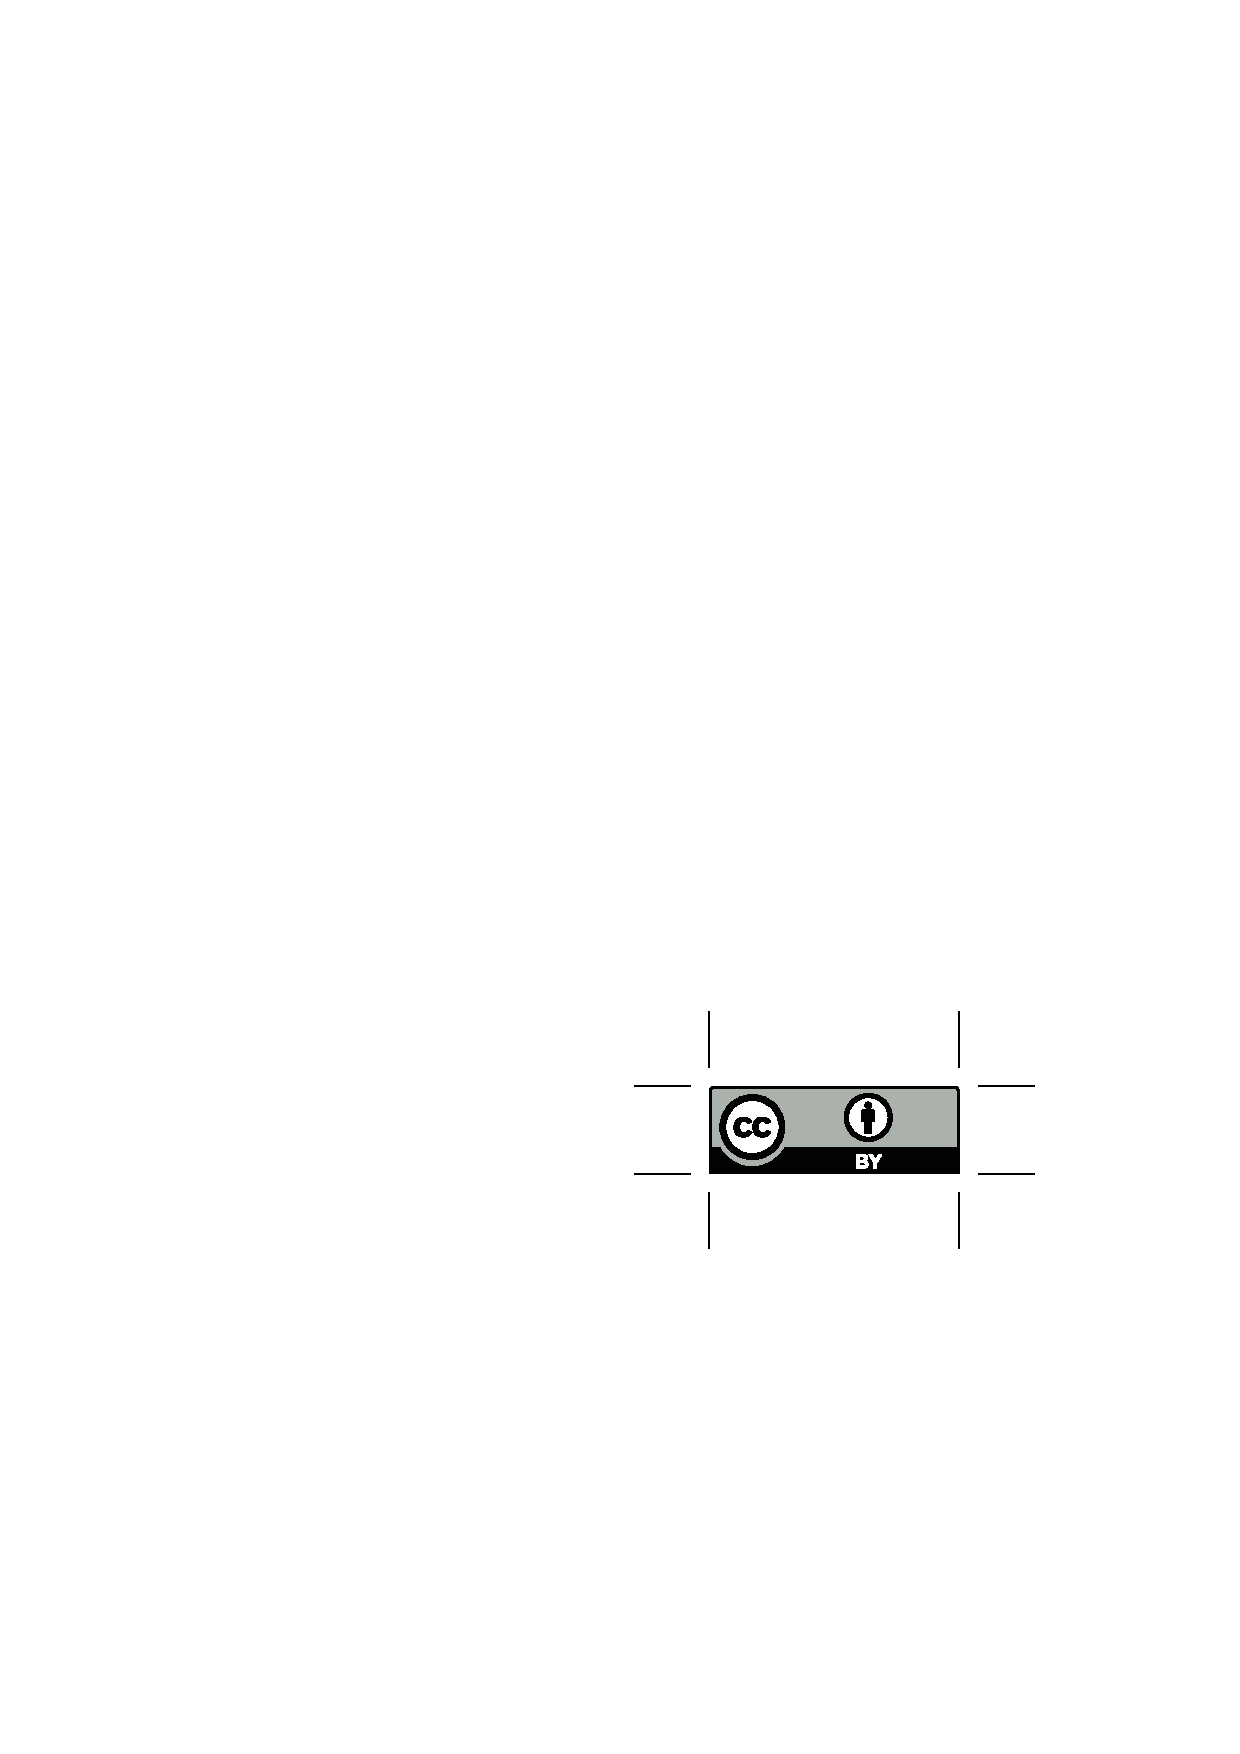
\includegraphics[width=0.90\textwidth]{by}}
  \end{minipage}\hfill
  \begin{minipage}{0.8\columnwidth}
   \href{https://creativecommons.org/licenses/by/4.0/}{This work is licensed under a Creative Commons Attribution International 4.0 License.}
  \end{minipage}
  \vspace{5pt}
}
\makeatother

\setcopyright{ifaamas}
\acmConference[AAMAS 2027]{Proc.\@ of the 26th International Conference
on Autonomous Agents and Multiagent Systems (AAMAS 2027)}{3--7 May 2027}{Hanoi, Vietnam}{M.~Baldoni, F.~Fang, W.~Yeoh, N.~Yorke-Smith (eds.)}
\copyrightyear{2027}
\acmYear{2027}
\acmDOI{}
\acmISBN{}
\acmSubmissionID{MASGym-2027-001}
\submissionType{Research Paper Track}

% ---- encoding / fonts ----
\usepackage[utf8]{inputenc}
\usepackage[T1]{fontenc}
\usepackage{microtype}
\usepackage{balance}

% ---- math ----
% NOTE: use amsfonts (not amssymb): acmart/sigconf loads newtxmath, and
% amssymb's \Bbbk redefinition conflicts with it.
\usepackage{amsmath,amsfonts,amsthm,mathtools,bm}
\usepackage{xspace}

% ---- citations (author--year, natbib is loaded by acmart) ----
\citestyle{acmauthoryear}

% ---- lists / tables / floats ----
\usepackage{enumitem}
\usepackage{booktabs,multirow,array}
\usepackage{xcolor}
\usepackage{float}

% ---- graphics: TikZ / PGFPlots ----
\usepackage{tikz}
\usetikzlibrary{arrows.meta,positioning,calc,fit,backgrounds,shapes.geometric,%
  shapes.symbols,decorations.pathreplacing,patterns,matrix,shadows.blur}
\usepackage{pgfplots}
\pgfplotsset{compat=1.18}
\usepgfplotslibrary{groupplots,fillbetween}

% ---- cross-document references (inert unless \externaldocument is used) ----
% Must be loaded before hyperref/cleveref resolve, hence its position here.
\usepackage{xr}

% ---- hyperlinks + clever references (hyperref is loaded by acmart) ----
\usepackage{cleveref}

% ---- shared TikZ styles (visual grammar) ----
% ============================================================================
% figures/tikz_styles.tex
% Shared visual grammar for all MASGym figures.
% Colour code (also encoded by shape/pattern for grayscale readability):
%   blue   = honest / normal system component (agents, orchestrator, memory)
%   orange/red = adversarial (colluders, compromised orchestrator, malicious tool, Sybil)
%   green  = defense / blue-team / deterministic checker (trusted evaluation)
%   purple = theory / mathematics
%   gray   = infrastructure / environment harness / background
% Arrow lanes: dataflow (blue), ctrlflow (gray dashed), advflow (red dashed),
%   defflow (green), theoryflow (purple).
% ============================================================================

% ---- palette ----
\definecolor{honest}{RGB}{31,97,164}      % blue
\definecolor{honestbg}{RGB}{219,232,246}
\definecolor{advers}{RGB}{200,63,42}      % red-orange
\definecolor{adversbg}{RGB}{250,224,216}
\definecolor{defense}{RGB}{34,139,80}     % green
\definecolor{defensebg}{RGB}{219,241,226}
\definecolor{theorycol}{RGB}{120,66,161}  % purple
\definecolor{theorybg}{RGB}{233,223,244}
\definecolor{infra}{RGB}{90,90,95}        % gray
\definecolor{infrabg}{RGB}{233,233,236}
\definecolor{amber}{RGB}{214,158,46}
\definecolor{amberbg}{RGB}{250,240,214}

% ---- generic node styles ----
\tikzset{
  >={Latex[length=2.4mm,width=1.8mm]},
  font=\small,
  block/.style={
    rounded corners=2pt, draw=infra!80, fill=infrabg, line width=0.7pt,
    align=center, inner sep=4pt, minimum height=8mm, text width=24mm},
  honestblock/.style={block, draw=honest!85, fill=honestbg, text=black},
  advblock/.style={block, draw=advers!85, fill=adversbg, text=black,
    dash pattern=on 3pt off 1.5pt},
  defblock/.style={block, draw=defense!80, fill=defensebg, text=black},
  theoryblock/.style={block, draw=theorycol!80, fill=theorybg, text=black},
  infrablock/.style={block, draw=infra!80, fill=infrabg},
  amberblock/.style={block, draw=amber!85, fill=amberbg, text=black},
  smalllabel/.style={font=\footnotesize, inner sep=1pt},
  arlbl/.style={midway, fill=white, inner sep=1.5pt, font=\scriptsize},
  % arrow "lanes"
  dataflow/.style={-{Latex[length=2.2mm]}, honest!85, line width=0.9pt},
  ctrlflow/.style={-{Latex[length=2.2mm]}, infra!85, line width=0.8pt,
    densely dashed},
  advflow/.style={-{Latex[length=2.2mm]}, advers!85, line width=1.0pt,
    dash pattern=on 3pt off 1.6pt},
  defflow/.style={-{Latex[length=2.2mm]}, defense!80, line width=1.0pt},
  theoryflow/.style={-{Latex[length=2.2mm]}, theorycol!80, line width=0.9pt},
  grp/.style={rounded corners=4pt, draw=#1!55, line width=0.8pt,
    fill=#1!5, inner sep=6pt},
  grp/.default=infra,
}

% ============================================================================
% Pure-TikZ icons (no external images, no fontawesome dependency).
% Each is a "pic" scaled to ~6mm; call with:  \pic at (x,y) {agenticon};
% ============================================================================

% -- worker agent (rounded robot head) --
\tikzset{
  agenticon/.pic={
    \draw[honest!85, fill=honestbg, line width=0.7pt, rounded corners=1pt]
      (-2.6mm,-2.2mm) rectangle (2.6mm,2.4mm);
    \draw[honest!85, fill=white, line width=0.5pt] (-1.2mm,0.3mm) circle (0.7mm);
    \draw[honest!85, fill=white, line width=0.5pt] (1.2mm,0.3mm) circle (0.7mm);
    \draw[honest!85, line width=0.6pt] (-1mm,-1.3mm) -- (1mm,-1.3mm);
    \draw[honest!85, line width=0.6pt] (0,2.4mm) -- (0,3.4mm);
    \fill[honest!85] (0,3.5mm) circle (0.5mm);
  }
}

% -- orchestrator (hub with crown) --
\tikzset{
  orchicon/.pic={
    \draw[honest!90, fill=honestbg, line width=0.8pt] (0,0) circle (2.7mm);
    \draw[honest!90, fill=honest!25, line width=0.6pt]
      (-2mm,0.6mm)--(-1mm,2.2mm)--(0,0.9mm)--(1mm,2.2mm)--(2mm,0.6mm)--(2mm,-0.4mm)--(-2mm,-0.4mm)--cycle;
    \fill[honest!90] (-2mm,0.6mm) circle (0.35mm);
    \fill[honest!90] (0,0.9mm) circle (0.35mm);
    \fill[honest!90] (2mm,0.6mm) circle (0.35mm);
  }
}

% -- compromised orchestrator (hub with crown + cross) --
\tikzset{
  orchbadicon/.pic={
    \draw[advers!90, fill=adversbg, line width=0.8pt] (0,0) circle (2.7mm);
    \draw[advers!90, fill=advers!20, line width=0.6pt]
      (-2mm,0.6mm)--(-1mm,2.2mm)--(0,0.9mm)--(1mm,2.2mm)--(2mm,0.6mm)--(2mm,-0.4mm)--(-2mm,-0.4mm)--cycle;
    \draw[advers!95, line width=0.9pt] (-1.2mm,-1.0mm)--(1.2mm,-2.4mm);
    \draw[advers!95, line width=0.9pt] (-1.2mm,-2.4mm)--(1.2mm,-1.0mm);
  }
}

% -- Byzantine / attacker node (warning cross) --
\tikzset{
  attackericon/.pic={
    \draw[advers!90, fill=adversbg, line width=0.8pt] (0,0) circle (2.7mm);
    \draw[advers!90, line width=0.9pt] (-1.3mm,-1.3mm)--(1.3mm,1.3mm);
    \draw[advers!90, line width=0.9pt] (-1.3mm,1.3mm)--(1.3mm,-1.3mm);
  }
}

% -- Sybil (two overlapping identity disks) --
\tikzset{
  sybilicon/.pic={
    \draw[advers!85, fill=adversbg, line width=0.7pt] (-1.1mm,0) circle (2.0mm);
    \draw[advers!85, fill=adversbg, line width=0.7pt] (1.1mm,0) circle (2.0mm);
    \draw[advers!85, line width=0.6pt] (-1.1mm,-0.4mm) circle (0.6mm);
    \draw[advers!85, line width=0.6pt] (1.1mm,-0.4mm) circle (0.6mm);
  }
}

% -- shield (defense / blue team) --
\tikzset{
  shieldicon/.pic={
    \draw[defense!85, fill=defensebg, line width=0.8pt]
      (0,3mm) -- (2.4mm,1.6mm) -- (2.4mm,-1mm) -- (0,-3mm)
      -- (-2.4mm,-1mm) -- (-2.4mm,1.6mm) -- cycle;
    \draw[defense!85, line width=0.9pt] (-1.1mm,0.2mm)--(-0.2mm,-1.2mm)--(1.4mm,1.2mm);
  }
}

% -- deterministic checker (clipboard + tick) --
\tikzset{
  checkericon/.pic={
    \draw[defense!85, fill=defensebg, line width=0.7pt, rounded corners=0.6pt]
      (-2mm,-2.7mm) rectangle (2mm,2.7mm);
    \draw[defense!85, fill=white, line width=0.5pt] (-0.9mm,2.3mm) rectangle (0.9mm,3.1mm);
    \draw[defense!85, line width=0.9pt] (-1.2mm,0.2mm)--(-0.3mm,-1.0mm)--(1.4mm,1.4mm);
  }
}

% -- LM tool emulator (cloud with function symbol) --
\tikzset{
  emuicon/.pic={
    \draw[infra!85, fill=infrabg, line width=0.7pt]
      (-2.4mm,-0.6mm) .. controls (-2.8mm,1.4mm) and (-0.9mm,1.9mm) .. (-0.6mm,1.2mm)
      .. controls (0.0mm,2.3mm) and (1.6mm,2.0mm) .. (1.5mm,0.9mm)
      .. controls (2.6mm,0.9mm) and (2.5mm,-0.8mm) .. (1.4mm,-0.9mm)
      -- (-2.0mm,-0.9mm) .. controls (-2.6mm,-0.9mm) and (-2.6mm,-0.6mm) .. (-2.4mm,-0.6mm) -- cycle;
    \node[infra!90, font=\scriptsize\itshape] at (0,0.1mm) {f};
  }
}

% -- tool (gear) --
\tikzset{
  toolicon/.pic={
    \draw[infra!85, fill=infrabg, line width=0.7pt] (0,0) circle (1.9mm);
    \foreach \a in {0,45,...,315}{
      \draw[infra!85, line width=0.8pt] (\a:1.9mm)--(\a:2.8mm);}
    \draw[infra!85, fill=white, line width=0.5pt] (0,0) circle (0.7mm);
  }
}

% -- malicious tool (gear, red, with cross) --
\tikzset{
  toolbadicon/.pic={
    \draw[advers!85, fill=adversbg, line width=0.7pt] (0,0) circle (1.9mm);
    \foreach \a in {0,45,...,315}{
      \draw[advers!85, line width=0.8pt] (\a:1.9mm)--(\a:2.8mm);}
    \draw[advers!90, line width=0.8pt] (-0.9mm,-0.9mm)--(0.9mm,0.9mm);
    \draw[advers!90, line width=0.8pt] (-0.9mm,0.9mm)--(0.9mm,-0.9mm);
  }
}

% -- shared memory store (cylinder/stack) --
\tikzset{
  memicon/.pic={
    \draw[honest!85, fill=honestbg, line width=0.7pt]
      (-2mm,-2.4mm) -- (-2mm,2mm) arc (180:0:2mm and 0.7mm) -- (2mm,-2.4mm)
      arc (0:-180:2mm and 0.7mm);
    \draw[honest!85, line width=0.6pt] (-2mm,2mm) arc (180:360:2mm and 0.7mm);
    \draw[honest!85, line width=0.5pt] (-2mm,0.4mm) arc (180:360:2mm and 0.7mm);
    \draw[honest!85, line width=0.5pt] (-2mm,-1.2mm) arc (180:360:2mm and 0.7mm);
  }
}

% -- poisoned memory (cylinder, red, droplet) --
\tikzset{
  membadicon/.pic={
    \draw[advers!85, fill=adversbg, line width=0.7pt]
      (-2mm,-2.4mm) -- (-2mm,2mm) arc (180:0:2mm and 0.7mm) -- (2mm,-2.4mm)
      arc (0:-180:2mm and 0.7mm);
    \draw[advers!85, line width=0.6pt] (-2mm,2mm) arc (180:360:2mm and 0.7mm);
    \fill[advers!80] (0,-0.2mm) circle (0.55mm);
  }
}

% -- neural net / model --
\tikzset{
  modelicon/.pic={
    \foreach \y in {-1.8mm,0mm,1.8mm}{\fill[honest!80] (-2.2mm,\y) circle (0.5mm);}
    \foreach \y in {-1mm,1mm}{\fill[honest!80] (0,\y) circle (0.5mm);}
    \fill[honest!80] (2.2mm,0) circle (0.5mm);
    \foreach \y in {-1.8mm,0mm,1.8mm}{\foreach \z in {-1mm,1mm}{
      \draw[honest!45, line width=0.3pt] (-2.2mm,\y)--(0,\z);}}
    \foreach \z in {-1mm,1mm}{\draw[honest!45, line width=0.3pt] (0,\z)--(2.2mm,0);}
  }
}

% -- database / dataset --
\tikzset{
  dbicon/.pic={
    \draw[infra!85, fill=infrabg, line width=0.7pt] (-2mm,-2.4mm) rectangle (2mm,2.4mm);
    \draw[infra!85, line width=0.6pt] (-2mm,1.2mm)--(2mm,1.2mm);
    \draw[infra!85, line width=0.6pt] (-2mm,0mm)--(2mm,0mm);
    \draw[infra!85, line width=0.6pt] (-2mm,-1.2mm)--(2mm,-1.2mm);
  }
}

% -- theorem scroll --
\tikzset{
  theoremicon/.pic={
    \draw[theorycol!80, fill=theorybg, line width=0.7pt, rounded corners=1pt]
      (-2mm,-2.6mm) rectangle (2mm,2.6mm);
    \draw[theorycol!80, line width=0.6pt] (-1.2mm,1.4mm)--(1.2mm,1.4mm);
    \draw[theorycol!80, line width=0.6pt] (-1.2mm,0.4mm)--(1.2mm,0.4mm);
    \draw[theorycol!80, line width=0.6pt] (-1.2mm,-0.6mm)--(0.6mm,-0.6mm);
  }
}

% -- human oversight (person) --
\tikzset{
  humanicon/.pic={
    \draw[infra!90, fill=infrabg, line width=0.7pt] (0,1.6mm) circle (1.0mm);
    \draw[infra!90, fill=infrabg, line width=0.7pt]
      (-1.6mm,-2.6mm) .. controls (-1.6mm,0.2mm) and (1.6mm,0.2mm) .. (1.6mm,-2.6mm) -- cycle;
  }
}

% ---- legend helper ----
\newcommand{\legendline}[2]{% #1 style, #2 text
  \draw[#1] (0,0) -- (5mm,0); \node[right, font=\scriptsize] at (5.5mm,0) {#2};}


% ============================================================================
% Theorem environments
% ============================================================================
\theoremstyle{plain}
\newtheorem{theorem}{Theorem}[section]
\newtheorem{lemma}[theorem]{Lemma}
\newtheorem{proposition}[theorem]{Proposition}
\newtheorem{corollary}[theorem]{Corollary}
\theoremstyle{definition}
\newtheorem{definition}[theorem]{Definition}
\newtheorem{assumption}{Assumption}
\theoremstyle{remark}
\newtheorem{remark}[theorem]{Remark}

\crefname{assumption}{Assumption}{Assumptions}
\Crefname{assumption}{Assumption}{Assumptions}

% ============================================================================
% Lightweight algorithm float + pseudocode macros
% (reproduce a numbered, ruled pseudocode listing with float.sty only)
% ============================================================================
\floatstyle{ruled}
\newfloat{algorithm}{tbp}{loa}
\floatname{algorithm}{Algorithm}
\crefname{algorithm}{Algorithm}{Algorithms}
\Crefname{algorithm}{Algorithm}{Algorithms}
\newcounter{algline}
\newlength{\algind}
\newcommand{\algreset}{\setcounter{algline}{0}\setlength{\algind}{0pt}}
\newcommand{\PL}[1]{\par\refstepcounter{algline}\noindent
  \makebox[2.6em][r]{\scriptsize\thealgline:\,}\hspace{0.5em}\hspace{\algind}%
  \ignorespaces#1\strut}
\newcommand{\Ind}{\addtolength{\algind}{1.5em}}
\newcommand{\Ded}{\addtolength{\algind}{-1.5em}}
\newcommand{\kw}[1]{\textbf{#1}}
\newcommand{\comm}[1]{\hfill{\footnotesize\itshape\color{black!55}\(\triangleright\)~#1}}

% ============================================================================
% Notation macros
% ============================================================================
\newcommand{\R}{\mathbb{R}}
\newcommand{\N}{\mathbb{N}}
\newcommand{\E}{\mathbb{E}}
\newcommand{\Prob}{\mathbb{P}}
\newcommand{\indic}{\mathbb{1}}
\newcommand{\Agents}{\mathcal{A}}          % set of agents
\newcommand{\Roles}{\mathcal{R}}           % role set
\newcommand{\Gtop}{\mathcal{G}}            % topology graph
\newcommand{\Vtop}{\mathcal{V}}
\newcommand{\Etop}{\mathcal{E}}
\newcommand{\Nin}{\mathcal{N}^{-}}          % inbound neighbourhood
\newcommand{\Trace}{\tau}                  % global state trace
\newcommand{\TraceSp}{\mathcal{T}}         % trace space
\newcommand{\Statesp}{\mathcal{S}}         % state space
\newcommand{\Predsec}{\Phi}                % system-level security predicate
\newcommand{\Predutil}{\Psi}               % benign-success predicate
\newcommand{\Checker}{\mathsf{C}}          % deterministic checker
\newcommand{\Emu}{\mathcal{E}_{\mathrm{LM}}} % LM tool emulator
\newcommand{\Judge}{\mathsf{J}}            % LLM judge (contrast)
\newcommand{\Advset}{\mathcal{B}}          % adversarial agent set
\newcommand{\betafrac}{\beta}              % adversary fraction
\newcommand{\config}{c}                    % environment configuration
\newcommand{\Configs}{\mathcal{C}}         % configuration space
\newcommand{\ASRs}{\mathrm{ASR}_{\mathrm{sys}}}
\newcommand{\ASRa}{\mathrm{ASR}_{\mathrm{act}}}
\newcommand{\PNAs}{\mathrm{PNA}_{\mathrm{sys}}}
\newcommand{\NRPs}{\mathrm{NRP}_{\mathrm{sys}}}
\newcommand{\CPR}{\mathrm{CPR}}            % compromise-propagation rate
\newcommand{\CSR}{\mathrm{CSR}}            % collusion success rate
\newcommand{\red}{\rho}                    % red policy
\newcommand{\blue}{\delta}                 % blue policy (defense)
\newcommand{\pinf}{p}                      % per-edge propagation probability
\newcommand{\thresh}{\theta}               % threshold (bootstrap percolation)
\newcommand{\kappaem}{\kappa}              % emulation agreement
\newcommand{\defname}{\textsc{MASGym}\xspace}
\newcommand{\corb}{\textsc{CoRB}\xspace}

% ============================================================================
% Title and author metadata (in the preamble, as in the official sample)
% ============================================================================
\title[MASGym: A Security Gym for Multi-Agent LLM Systems]{\defname: A
Co-Evolving Red/Blue Security Gym for Multi-Agent LLM Systems with
Parameterized Collusion, Orchestrator Compromise, and System-Level Metrics}

% Anonymous double-blind submission: the author block is suppressed by the
% `anonymous' class option. For camera-ready, remove that option and fill in
% your full author list, affiliations, and emails.
\author{Thanh Pham}
\affiliation{%
  \institution{School of Computing Technologies, RMIT University}
  \country{Melbourne, Australia}}
\email{thanhphamchivn@gmail.com}

% Abstract and keywords must be defined in the preamble, before \maketitle.
\begin{abstract}
The strongest existing LLM-agent security benchmarks---Agent Security Bench, AgentDojo,
InjecAgent, ToolEmu---are single-agent, yet deployed systems are collectives in which a
planner directs workers, agents share memory, and tools are third-party. The phenomena
that dominate risk there---collusion, a compromised orchestrator, malicious tools, Sybils,
group-level emergent failure---cannot be produced by a single-agent harness. We present
\defname{}, an environment and evaluation methodology for multi-agent LLM security: a
forced-coordination task suite with heterogeneous roles and partial observability over star,
chain, tree, and mesh topologies at $3$--$50$ agents; a parameterized adversary model; a
system-level metric $\NRPs=\PNAs(1-\ASRs)$ scored by a deterministic checker over the global
state trace, never an LLM judge on the critical path; and \corb, a co-evolving red/blue
protocol logging attack--defense trajectories and a (security, cost) Pareto frontier.
Supporting theory, proved under explicit assumptions, characterizes the metric
axiomatically (reducing to ASB at one agent), bounds compromise propagation across
topologies, establishes a strict collusion advantage and a forced-coordination lower bound,
and proves evaluator integrity. On a clearly-labelled \emph{synthetic} emulator, a
per-agent guardrail's relative ASR reduction shrinks
$41.6\%\to31.8\%\to27.6\%$ from single-agent to collusion to compromised-orchestrator
context. We then ask what that guardrail buys, and answer on four real backbones in three
model families: a prompt-level defense drives action-channel compliance to $0/1075$
decisions, so $\ASRa{=}0$ throughout, yet $\ASRs$ remains $1.000$ on tree and star,
because once the unsafe action is blocked the system predicate is still discharged by
deterministic availability sabotage that topology alone determines. A fourth backbone
ignores the defense entirely. A defense measured on the action channel therefore cannot
certify system-level security, and its efficacy is a property of the model as much as of
the defense.
\end{abstract}

\keywords{multi-agent LLM security; security benchmark; co-evolving red/blue evaluation;
collusion; prompt injection; deterministic security checking; system-level metrics}


\begin{document}


\maketitle

% ---------------------------------------------------------------------------
% Body
% ---------------------------------------------------------------------------
\section{Introduction}
\label{sec:intro}

Progress in the security of large language model (LLM) agents has tracked the quality of
the instruments used to measure it. Agent Security Bench
(ASB)~\cite{zhang2025asb} introduced a utility--security metric
$\mathrm{NRP}=\mathrm{PNA}\cdot(1-\mathrm{ASR})$; AgentDojo~\cite{debenedetti2024agentdojo}
evaluates an agent under injection with \emph{deterministic}, state-based
\texttt{security()} checks; ToolEmu~\cite{ruan2024toolemu} emulates arbitrary tool
execution; InjecAgent~\cite{zhan2024injecagent} benchmarks indirect injection. These
instruments are strong but single-agent: their only cross-agent channel is a shared memory
store. Yet deployed systems such as AutoGen~\cite{wu2023autogen},
MetaGPT~\cite{hong2023metagpt}, CAMEL~\cite{li2023camel},
ChatDev~\cite{qian2024chatdev}, and Magentic-One~\cite{fourney2024magenticone} are
orchestrated \emph{collectives}: a planner directs workers, agents share memory,
third-party tools sit on the critical path, and many tasks require several agents to
finish at all.

In such systems the security questions are group-level. Do a fraction of agents
\emph{collude}? Is the \emph{orchestrator} trusted, or compromised? Can a \emph{malicious
tool}, a \emph{Sybil} identity, or a \emph{poisoned} memory entry spread through the
collective? Re-running a single-agent benchmark $N$ times cannot produce these phenomena.
MASEC~\cite{schroederdewitt2025masec} argues that agent security is
\emph{non-compositional}---individually safe agents compose into unsafe systems---and
notes that no multi-agent security benchmark exists, listing what one must provide:
heterogeneous roles, partial observability, forced coordination, a co-evolving red/blue
methodology, and group-level emergence metrics.

\paragraph{Contributions.}
To the best of our knowledge \defname{} is the first environment purpose-built for the
security of multi-agent LLM systems. It is not a new attack or defense; it is an
environment and evaluation methodology whose scientific object is the controlled variation
of coordination, collusion, and orchestrator variables and the system-level metrics that
quantify their effect (architecture in the Supplementary Material; three-layer design in
\Cref{sec:method}). Concretely,
\begin{itemize}[leftmargin=1.4em]
\item \textbf{An environment and task suite} (\Cref{sec:system,sec:method}): heterogeneous
roles, partial observability, \emph{forced-coordination} tasks (no agent can complete one
alone), over star/chain/tree/mesh topologies at $3$--$50$ agents.
\item \textbf{A parameterized adversary model} (\Cref{sec:threat}): one vector controls
adversary fraction, collusion, adaptivity, orchestrator compromise, malicious tools,
Sybils, and poisoned memory, under a system-level compromise objective.
\item \textbf{A system-level metric suite} (\Cref{sec:problem,sec:method}): the
generalization $\NRPs=\PNAs(1-\ASRs)$, scored by a \emph{deterministic checker} over the
global trace so an injection cannot hijack the evaluator (\Cref{thm:integrity}), plus
collusion-success and compromise-propagation rates, coordination quality, cost, and
recovery.
\item \textbf{The \corb{} co-evolving red/blue protocol} (\Cref{sec:algorithm}), logging
$(\text{attack},\text{defense},\NRPs)$ trajectories and a (security, cost) Pareto frontier.
\item \textbf{An answer to ``does the defense work?''} (\Cref{sec:defense}): on four real
backbones in three model families a prompt-level defense drives action-channel compliance
to $0/1075$ decisions---$\ASRa{=}0$---yet $\ASRs$ stays $1.000$ on tree and star, because
the residual failure is deterministic availability sabotage that topology alone determines,
and one backbone ignores the defense entirely (\Cref{tab:defense}). A defense scored on the
action channel cannot certify system-level security. The controlled synthetic sweep
separately measures the guardrail's shrinking margin, $41.6\%\to31.8\%\to27.6\%$
(degradation grid, Supplementary Material).
\end{itemize}

Because reviewers rightly discount benchmarks whose central metric is asserted rather than
justified, we treat theory as part of the instrument (\Cref{sec:theory}): under explicit
assumptions and honest proof-status labels we prove the product aggregator is the unique
combiner satisfying our axioms and reduces to ASB at $N{=}1$; that the deterministic
checker cannot be hijacked through message content, unlike a message-reading LLM judge,
which we measure pushed off the recorded state in roughly a third of injected traces;
topology-dependent propagation bounds and a strict collusion advantage in the cascade
model; a forced-coordination lower bound; and finite-sample concentration. None
asserts that any real defense is secure or provably degrades.

\paragraph{Scope and stance.}
\defname{} is an instrument, not a verdict: a lower $\ASRs$ is a measurement under a stated
configuration, not a certificate. The central threat to validity is emulation
fidelity---ToolEmu's reported human agreement is $\kappaem\approx0.48$---so scoring routes
through the deterministic checker, the caveat is explicit, and the harness registers
emulated-versus-real ablations for independent re-testing. Of those two we ran the
deterministic-versus-judge half on real judge backbones (\Cref{sec:integrity}); the
emulated-versus-real-tools half is unmeasured, since no real tool backend is wired in.
The checker and harness form a trusted computing base, and model-weight attacks are out
of scope. Roadmap:
\Cref{sec:related}--\Cref{sec:prelim} situate and fix notation; \Cref{sec:system,sec:threat,sec:problem}
formalize; \Cref{sec:method,sec:algorithm} present the environment and protocol;
\Cref{sec:theory} justifies; \Cref{sec:experiments} evaluates; the final sections discuss and
bound limitations.
\section{Related Work}
\label{sec:related}

\subsection{Single-agent security instruments}
The closest instruments evaluate a lone tool-using agent. ASB~\cite{zhang2025asb}
formalizes attacks and defenses for agents and introduces the utility--security metric
$\mathrm{NRP}=\mathrm{PNA}\cdot(1-\mathrm{ASR})$ that we generalize; its threat model is
single-agent with retrieved memory. AgentDojo~\cite{debenedetti2024agentdojo} contributes
a stateful environment whose \emph{deterministic} security/utility functions are computed
from pre- and post-execution state, so a prompt injection cannot also hijack the evaluator;
it names multi-agent planner/worker defense as future work.
InjecAgent~\cite{zhan2024injecagent}, ToolEmu~\cite{ruan2024toolemu},
AgentHarm~\cite{andriushchenko2025agentharm}, HarmBench~\cite{mazeika2024harmbench}, and
formalizations of prompt injection~\cite{liu2024formalizing} and
trustworthiness~\cite{wang2023decodingtrust} complete the single-agent picture. None
parameterizes collusion, orchestrator trust, Sybils, or compromise propagation.

\subsection{Multi-agent LLM frameworks and attacks}
A large literature builds collectives---AutoGen~\cite{wu2023autogen},
MetaGPT~\cite{hong2023metagpt}, CAMEL~\cite{li2023camel},
ChatDev~\cite{qian2024chatdev}, Magentic-One~\cite{fourney2024magenticone}, and
mixing/debating designs~\cite{du2023debate}---concerned with capability, not security;
\defname{} adopts their role structures as substrate. A fast-growing attack literature is
intrinsically multi-agent: prompt infection~\cite{lee2024promptinfection},
contagious blocking~\cite{zhou2025corba}, population jailbreaking~\cite{gu2024agentsmith},
topological safety~\cite{yu2024netsafe}, adversarial roles~\cite{tian2023evilgeniuses},
GenAI worms~\cite{cohen2024aiworm}, memory poisoning~\cite{chen2024agentpoison}, and
backdoors~\cite{yang2024watchout}. These are attacks in bespoke setups; \defname{} is the
controlled, deterministically scored environment in which such attacks and defenses can be
swept and compared.

\subsection{Defenses, surveys, and systematizations}
Multi-agent defenses include AutoDefense~\cite{zeng2024autodefense} and the
topology-guided G-Safeguard~\cite{yu2025gsafeguard}; per-agent guardrails
(TrustAgent~\cite{hua2024trustagent}, Llama Guard~\cite{inan2023llamaguard}, NeMo
Guardrails~\cite{rebedea2023nemo}) are the baselines we lift into the collective setting.
Classical Byzantine fault tolerance~\cite{lamport1982byzantine,pease1980reaching} and
Byzantine-robust aggregation~\cite{blanchard2017krum} tolerate faulty fractions under a
trusted coordinator over numeric messages; they motivate our collusion and
orchestrator-trust knobs without covering natural-language collectives. Surveys of
agent security~\cite{he2025emerged,li2024personalllmagents} and the
non-compositionality argument~\cite{schroederdewitt2025masec,hammond2025multiagent} are the
gap \defname{} addresses.

\subsection{Environments, red teaming, and evaluation validity}
Methodologically \defname{} follows standardized environments---Gym~\cite{brockman2016openaigym},
PettingZoo~\cite{terry2021pettingzoo}, and Melting Pot~\cite{leibo2021meltingpot}, which
evaluates social outcomes at the level of the collective---and automated red
teaming~\cite{perez2022redteaming}, with the MAST taxonomy~\cite{cemri2025mast}
supplying a vocabulary for group-level failures. On scoring validity, LLM-as-judge
evaluation is documented as manipulable and biased~\cite{zheng2023judging,wang2023fair};
\defname{} therefore keeps a deterministic trace-based checker on the critical path and
treats the deterministic-versus-judge comparison as a measurable ablation.

\subsection{Positioning}
\defname{} is \emph{not} ASB applied to many agents (ASB's only cross-agent vector is
shared memory), \emph{not} AgentDojo at scale (its deterministic checker is per-agent over
environment state; a collective requires system-level predicates over a global trace,
\Cref{sec:problem}), and \emph{not} a model-swap or prompt-filter study: its object is the
controlled variation of coordination, collusion, and orchestrator variables, and the
system-level metrics that quantify their effect.
\section{Preliminaries and Notation}
\label{sec:prelim}

This section recalls the three primitives \defname{} builds on (notation summarized in the
Supplementary Material): ASB's utility--security metric, AgentDojo's
deterministic state-based checking, and ToolEmu's LM tool emulation.

\subsection{ASB's utility--security metric}
ASB~\cite{zhang2025asb} scores an agent by a \emph{Non-Refusal Performance},
\begin{equation}
\label{eq:asb-nrp}
\mathrm{NRP} \;=\; \mathrm{PNA}\cdot(1-\mathrm{ASR}),
\end{equation}
where $\mathrm{PNA}\in[0,1]$ is performance on benign tasks and $\mathrm{ASR}\in[0,1]$ the
attack success rate; the product rewards a system only when both useful and not attacked.
\Cref{eq:asb-nrp} is defined for a single agent; generalizing it to a collective is the
subject of \Cref{sec:problem,sec:theory}.

\subsection{AgentDojo's deterministic state-based checking}
AgentDojo~\cite{debenedetti2024agentdojo} evaluates security by \emph{deterministic}
functions of environment state rather than an LLM judge: a task fixes a predicate reading
the pre- and post-execution state and returning a Boolean, so an injection cannot
manipulate the score unless it changes the security-relevant state. \defname{} lifts this
property to the system level: our checker $\Checker$ evaluates $\Predsec,\Predutil$ over the
\emph{global} trace $\Trace$, never an invocable LLM judge, and we prove the resulting
integrity property in \Cref{thm:integrity}.

\subsection{ToolEmu's LM tool emulation}
ToolEmu~\cite{ruan2024toolemu} emulates tool execution from a specification with a language
model, enabling breadth at low cost, at a reported human agreement of only
$\kappaem\approx0.48$ (Cohen's $\kappa$~\cite{cohen1960coefficient}, extended to many
raters by Fleiss~\cite{fleiss1971measuring}). \defname{} adopts LM emulation for tool
breadth, including an adversarial mode $\Emu^{\!\dagger}$ for malicious tools, but treats
$\kappaem$ as a first-class threat to validity: scoring routes through the deterministic
  checker, and the harness registers an emulated-versus-real-tools ablation for
  independent re-testing. We did not run it: no real tool backend is wired into our
  environment, so we report it as an unmeasured gap rather than let the registration
  imply coverage (\Cref{sec:limitations}). An \emph{episode} runs a task under a fixed configuration
$\config$ and produces a global trace $\Trace\sim\mathcal{D}(\config)$, from which all
security and utility quantities are computable---the fact that makes deterministic,
hijack-resistant scoring possible.

% Notation table moved to the Supplementary Material to keep the main paper
% within its page limit; main-text references it in prose.
\section{System Model}
\label{sec:system}

\defname{} evaluates a collective of $N\in\{3,\dots,50\}$ LLM agents
$\Agents=\{a_1,\dots,a_N\}$, each assigned exactly one role from the set $\Roles$
(notation in the Supplementary Material). Roles pool access to shared tools and a shared
versioned memory, and interplay is \emph{structural}, captured by a topology
$\Gtop=(\Vtop,\Etop)$ over agents---star, chain, tree, or mesh---that fixes who may
influence whom:
$j\in\Nin(a)$ means $a$ reads $j$'s outputs; the orchestrator is typically the star's
centre.

An \emph{episode} executes a task under a configuration $\config$ for $H$ steps, producing
a \emph{global trace} $\Trace=(s_0,\dots,s_H)$, where $s_t$ is the complete state: every
agent's messages, tool calls, tool outputs, memory versions, role assignments, topology
edges, and the agent-identity map. Traces are i.i.d.\ from $\mathcal{D}(\config)$
(\Cref{as:iid}). Because $\Predsec,\Predutil$ are functions of recorded state only
(\Cref{def:predicates}), system-level quantities are computable offline from $\Trace$,
which is what keeps the checker deterministic and the measurement reproducible. A
configuration $\config\in\Configs$ specifies task, $\Gtop$, models, tools, $\Advset$, and
protocol constants, so a study reports $\NRPs$ as a coordinate over a \emph{sweep} that
varies exactly one component at a time under a controlled seed.

\section{Threat Model}
\label{sec:threat}

The adversary is a \emph{set} $\Advset\subseteq\Agents$ of \emph{adversarial agents},
of size $\betafrac N$ chosen by the operator---a single corrupted node or a coordinated
coalition sharing a channel and a joint objective. Capabilities and attack mode are fixed
by
\begin{equation}
\label{eq:adv-config}
\config_{\mathrm{adv}}\;=\;\bigl(\betafrac,\ \mathsf{coll},\ \mathsf{adapt},\ \mathsf{orch},\ \mathsf{tool},\ \mathsf{syb},\ \mathsf{mem}\bigr),
\end{equation}
selecting respectively: adversary fraction; independent vs.\ colluding coordination
(\Cref{def:csr}); static vs.\ adaptive attacks across \corb{} rounds; compromised
orchestrator; malicious tools (adversarial emulator $\Emu^{\!\dagger}$); Sybils; and
poisoned memory. $\Advset$ may issue messages and tool calls as its roles, read
$\mathcal{M}$, and read the outputs of its topology predecessors; \emph{outside} its
powers are the harness, the recorded trace, the checker, the emulator's mechanism, and the
honest agents' private internals. Compromise then \emph{propagates} along $\Gtop$
(\Cref{def:propagation}) from these seeds, so the effective compromised set at episode end,
$\Advset_\infty$, can exceed $\Advset$.

\textbf{Inferential threats and scope.} The operator sets horizon, models, and metrics; the
adversaries do not. An \emph{LLM judge}, when used (only in ablations, off the critical
path), is a \emph{measurement} threat: human agreement is $\kappaem\approx0.48$ and judges
can be gamed; the deterministic checker exists to remove this threat (\Cref{thm:integrity},
\Cref{prop:judgehijack}). The TCB is the harness (trace recording, roles, topology,
scheduling), the tool specifications, and the registered predicates; everything
else---messages, memory writes, tool outputs, intent---is outside the TCB. Scope is
\emph{per se} the \emph{collective}; adversaries are bounded by the seven knobs and episodic
budgets; a harness-level adversary and model-weight attacks are out of scope; honest agents
have no budget (per ASB) and obey their assigned roles.
% Threat Model section is merged into system_model.tex to save body pages.
% Historical reference: sec:threat now labels the merged section there.
\section{Problem Formulation}
\label{sec:problem}

We define what a system-level security benchmark must measure: security and benign-success
predicates, the system-level metric aggregating them, and the group-level quantities
(forced coordination, compromise propagation, collusion) with no single-agent analogue.

\subsection{System-level predicates}
\begin{definition}[System-level security and benign-success predicates]
\label{def:predicates}
A task fixes two Boolean functionals of the global trace $\Trace\in\TraceSp$: a
\emph{security predicate} $\Predsec:\TraceSp\to\{0,1\}$, $1$ iff the trace contains a
system-level compromise (an unsafe action executed, protected data exfiltrated, or a
forced-coordination task sabotaged), and a \emph{benign-success predicate}
$\Predutil:\TraceSp\to\{0,1\}$, $1$ iff the collective completed the legitimate task.
Both are registered programs evaluated by the deterministic checker over the
harness-recorded trace; dependencies on \emph{un}-recorded natural-language content are
disallowed, yielding evaluator integrity (\Cref{thm:integrity}) and lifting
AgentDojo~\cite{debenedetti2024agentdojo} from one agent's state to the global trace.
\end{definition}

\subsection{System-level metrics}
\begin{definition}[System-level ASR, PNA, and NRP]
\label{def:metrics}
Fix a configuration $\config$ and let $\Trace\sim\mathcal{D}(\config)$. Define
\begin{align}
\ASRs(\config) &\;=\; \Prob_{\Trace\sim\mathcal{D}(\config)}\!\bigl[\Predsec(\Trace)=1\bigr],
\label{eq:asrsys}\\
\PNAs(\config) &\;=\; \Prob_{\Trace\sim\mathcal{D}(\config^{\circ})}\!\bigl[\Predutil(\Trace)=1\bigr],
\label{eq:pnasys}\\
\NRPs(\config) &\;=\; \PNAs(\config)\cdot\bigl(1-\ASRs(\config)\bigr),
\label{eq:nrpsys}
\end{align}
where $\config^{\circ}$ is $\config$'s benign counterpart (no adversary), so $\PNAs$ measures
coordinated-task performance uncontaminated by attack-induced refusals, exactly as ASB
separates PNA from ASR.
\end{definition}

Two properties are required and proved in \Cref{sec:theory}: \Cref{eq:nrpsys} \emph{reduces}
to ASB's \Cref{eq:asb-nrp} at $N{=}1$ (\Cref{prop:reduction}), and the product form is
\emph{justified} rather than assumed, via an axiomatic characterization over D1--D5
(\Cref{sec:theory}; \Cref{thm:metric}). The benchmark stance: $\NRPs$ is a coordinate for
comparing configurations, not a certificate.

\subsection{Forced coordination}
\begin{definition}[$k$-forced-coordination task]
\label{def:forced}
For an agent set $\Agents$, let a \emph{witness} be a set $W\subseteq\Agents$ whose joint
contributions can satisfy $\Predutil$. A task is \emph{$k$-forced-coordination} if every
witness has size $|W|\ge k$; equivalently, for every $S$ with $|S|<k$, no assignment in
which only the agents of $S$ act non-trivially satisfies $\Predutil$.
\end{definition}

$k$-forced tasks with $k\ge2$ cannot be represented in a single-agent harness.
\Cref{sec:theory} relates task disruption to whether $\Advset$ intersects every minimal
witness (a hitting-set condition, \Cref{prop:forced}).

\subsection{Compromise propagation and collusion}
\begin{definition}[Compromise relation and propagation rate]
\label{def:propagation}
Let $\Advset_0=\Advset$ be the initially adversarial (seed) agents. Compromise spreads
over $\Gtop$ according to a monotone rule $\mathcal{P}$ (\Cref{sec:theory}: an
independent-cascade model with per-edge probability $\pinf$, or a threshold model with
threshold $\thresh$). Write $\Advset_\infty\supseteq\Advset_0$ for the compromised set at
fixation. The \emph{compromise-propagation rate} is
\begin{equation}
\label{eq:cpr}
\CPR(\config) \;=\; \E\!\left[\frac{|\Advset_\infty|-|\Advset_0|}{\,N-|\Advset_0|\,}\right],
\end{equation}
the expected fraction of \emph{initially honest} agents that become compromised.
\end{definition}

\begin{definition}[Collusion success rate]
\label{def:csr}
For a fixed fraction $\betafrac$, let $\ASRs^{\mathrm{coll}}$ and $\ASRs^{\mathrm{ind}}$ be
the system attack success rates under colluding and independent adversaries respectively.
The \emph{collusion success rate} reports $\ASRs^{\mathrm{coll}}$, and the
\emph{collusion advantage} is $\Delta_{\mathrm{coll}}=\ASRs^{\mathrm{coll}}-\ASRs^{\mathrm{ind}}$.
\end{definition}
\section{The \defname{} Environment}
\label{sec:method}

\defname{} is organized as three layers (architecture figure in the Supplementary Material): an \emph{emulation
layer} that supplies tools, a \emph{deterministic checking layer} that scores
system-level predicates, and an \emph{orchestration layer} that instantiates the system
and threat models and drives the \corb{} loop.

% moved to Supplementary Material (page limit): see \Cref{fig:architecture} there.
% \input{figures/tikz_architecture.tex}

\subsection{Emulation and deterministic checking}
Following ToolEmu~\cite{ruan2024toolemu}, tool execution is emulated by a language model
$\Emu$ from a tool specification, giving breadth without hand-built sandboxes; an
\emph{adversarial} mode $\Emu^{\!\dagger}$ realizes malicious tools (attacker-controlled
responses, exfiltration bait, injected instructions). Crucially the emulator is \emph{not}
on the scoring critical path: it produces the tool outputs agents consume, while the
verdict comes from the deterministic checker, so emulator noise degrades realism, not
scoring integrity. The checker $\Checker$ evaluates the registered predicates
$\Predsec,\Predutil$ over the global trace (\Cref{def:predicates}) and never invokes an
LLM judge on the critical path. Predicates are programs over recorded state: an
\emph{exfiltration} predicate fires iff protected data recorded as leaving the trust
boundary appears in an outbound tool call; a \emph{sabotage} predicate fires iff a
$k$-forced task's witness set was prevented from completing; an \emph{unsafe-action}
predicate fires iff a denylisted transition is recorded. An optional LLM judge\nobreak\
$\Judge$, available only off the critical path, enables the ablation (RQ2).

\subsection{Orchestration layer and task suite}
The orchestration layer builds the topology $\Gtop$, assigns roles, enforces observability
masks, applies $\config_{\mathrm{adv}}$ of \Cref{eq:adv-config}, and runs episodes; it is
part of the TCB and exposes the \corb{} interface (\Cref{sec:algorithm}). Tasks are
\emph{forced-coordination} by design (\Cref{def:forced}), so the collective is the unit of
analysis: each provides a benign goal decomposable across roles, a registered pair
$(\Predutil,\Predsec)$, a tool set (some malicious under $\mathsf{tool}$), a shared-memory
schema (poisonable under $\mathsf{mem}$), and a topology (star: hub-and-spoke delegation;
chain: pipelines; tree: hierarchical; mesh: peer collaboration), parameterized by $k$ (the
degree of forced coordination) and benign difficulty.

\subsection{Realized adversary knobs}
Each component of $\config_{\mathrm{adv}}$ maps to a concrete harness mechanism:
$\betafrac$ selects the seed set $\Advset$; $\mathsf{coll}$ toggles a shared channel and
joint objective; $\mathsf{adapt}$ enables red co-evolution across \corb{} rounds;
$\mathsf{orch}$ flips the orchestrator's policy; $\mathsf{tool}$ routes tools through
$\Emu^{\!\dagger}$; $\mathsf{syb}$ instantiates extra identities under one controller; and
$\mathsf{mem}$ writes poisoned entries to shared memory. Because the knobs are independent,
a study isolates each variable's effect while holding the rest fixed---the controlled
variation that is the paper's scientific object~\cite{rubin1974estimating}.

\subsection{Metric suite}
\label{sec:metric-suite}
All reported quantities are computed from traces by the deterministic checker or harness
logs; none is an LLM-judge verdict: system attack success rate $\ASRs$ and system NRP
$\NRPs$ (\Cref{eq:asrsys,eq:nrpsys}); benign performance $\PNAs$ (\Cref{eq:pnasys});
collusion success rate and advantage (\Cref{def:csr}); compromise-propagation rate $\CPR$
(\Cref{eq:cpr}); coordination quality and its degradation under sabotage; time-to-detection
and recovery; token/API cost and latency and their scaling with $N$; and human-intervention
rate. Estimating these to target precision requires the budget fixed by \Cref{thm:sample};
the resulting cost model---$\Theta(MNH)$ agent invocations per configuration,
$\Theta(GNH\Delta^{-2}\ln(G/\alpha))$ for a sweep---is reported with each study and
archived in full with the harness.
\section{The \corb{} Co-Evolving Red/Blue Protocol}
\label{sec:algorithm}

\defname{}'s evaluation methodology is a co-evolving loop, \corb, that alternates a red
policy proposing attack configurations and a blue policy proposing defenses, scoring each
pair with the deterministic checker and logging a trajectory of
$(\text{attack},\text{defense},\NRPs)$ triples. The per-configuration scoring procedure
(\textsc{ScoreConfig}) is fully specified: instantiate $\Gtop$, roles, masks, and the
adversary knobs $\config_{\mathrm{adv}}$\Cref{eq:adv-config} via the trusted harness; seed
$\Advset_0$; run $M$ episodes of $H$ steps, recording each transition into the global
trace and updating the compromised set under the propagation rule $\mathcal{P}$
(\Cref{def:propagation}); evaluate $(\Predutil,\Predsec)$ with the deterministic checker on
each trace; and aggregate $\widehat{\ASRs},\widehat{\PNAs},\widehat{\NRPs},\widehat{\CPR}$
plus detection and recovery statistics. The protocol-level loop is \Cref{alg:corb}. Both
levels keep the LLM off the scoring critical path, so no proposal can inflate its own
score.

\begin{algorithm}[t]
\caption{\corb: co-evolving red/blue evaluation.}
\label{alg:corb}
\algreset
\PL{\kw{Input:} red policy $\red$; blue policy $\blue$; rounds $R$; task, budget $M$.}
\PL{\kw{Output:} trajectory $\mathcal{L}=\{(\config^r_{\mathrm{adv}},\blue^r,\NRPs^r,\ASRs^r)\}_{r=1}^R$
and a Pareto frontier.}
\PL{Initialize defense $\blue^0$ (no-defense or a lifted per-agent defense).}
\PL{\kw{for} $r=1,\dots,R$ \kw{do}}\Ind
\PL{\emph{Red step:} $\config^r_{\mathrm{adv}}\gets\red(\mathcal{L}_{<r},\blue^{r-1})$
\comm{static: fixed; adaptive: best-response}}
\PL{Score $(\config^r_{\mathrm{adv}},\blue^{r-1})$ with \textsc{ScoreConfig}.}
\PL{\emph{Blue step:} $\blue^r\gets\blue(\mathcal{L}_{<r},\config^r_{\mathrm{adv}})$
\comm{propose/upgrade defense}}
\PL{Re-score $(\config^r_{\mathrm{adv}},\blue^r)$; append both scorings to $\mathcal{L}$.}\Ded
\PL{\kw{return} $\mathcal{L}$ and its $(\ASRs,\text{cost})$ / $(\NRPs,\text{cost})$ frontier.}
\end{algorithm}

Three properties make \corb{} a measurement protocol rather than a training loop:
(i) \emph{integrity}---every score comes from \textsc{ScoreConfig}, so neither policy can
hijack its own evaluation (\Cref{thm:integrity}); (ii) \emph{reproducibility}---the
trajectory $\mathcal{L}$ is the full audit trail of fully specified
$(\config_{\mathrm{adv}},\blue)$ pairs; and (iii) \emph{honesty of the frontier}---\corb{}
reports a Pareto frontier over (security, cost) rather than a single ``winner''. The red
and blue policies may be grid/random search, an optimizer, or an LLM-driven proposer;
\defname{} fixes the \emph{interface} and the \emph{scoring}, not the proposers. Cost is
$\Theta(RMNH)$ for an $R$-round run and $\Theta(GNH\Delta^{-2}\ln(G/\alpha))$ across a
$G$-configuration sweep (\Cref{cor:budget}).
\section{Theory: What the Instrument Measures}
\label{sec:theory}

A benchmark earns trust when its central metric is justified, its evaluator cannot be
gamed, and its sample sizes are principled. We therefore treat theory as part of the
instrument. All results are stated under explicit assumptions (below) and carry honest
proof-status labels; none claims that any real defense is secure or provably degrades.
Short proofs of the central characterization and integrity theorems are inline; remaining
derivations and the complete proof archive ship with the harness (Supplementary Material).

\begin{assumption}[Trusted checking]
\label{as:tcb}
The harness records a faithful global trace $\Trace$, and the checker $\Checker$
evaluates the fixed predicates $\Predsec,\Predutil$ as functions of $\Trace$ \emph{only}
(\Cref{def:predicates}).
\end{assumption}
\begin{assumption}[i.i.d.\ episodes]
\label{as:iid}
For fixed $\config$, the $M$ episode traces are independent draws from
$\mathcal{D}(\config)$.
\end{assumption}
\begin{assumption}[Bounded indicators]
\label{as:bounded}
$\Predutil,\Predsec\in\{0,1\}$.
\end{assumption}
\begin{assumption}[Monotone propagation model]
\label{as:prop}
Compromise spreads over $\Gtop$ via a monotone rule $\mathcal{P}$ (\Cref{def:propagation}):
under \emph{independent cascade}, a compromised agent independently compromises each
susceptible out-neighbour with probability $\pinf$; under \emph{threshold}, a susceptible
agent is compromised once at least $\thresh$ in-neighbours are. This is a modelling choice
\defname{} makes so propagation is measurable, not an empirical law; its realism is itself
measured via $\CPR$.
\end{assumption}
\begin{assumption}[Continuity of the aggregator]
\label{as:cont}
The utility--security aggregator $g:[0,1]^2\to[0,1]$ is continuous.
\end{assumption}

\subsection{Characterization of the system-level metric}
\label{sec:theory-metric}
The product form of $\NRPs$ is forced by the desiderata of \Cref{sec:problem}, phrased as
five axioms (D1--D5): boundedness, consistency, monotonicity, homogeneity (each in both
arguments), and reduction---the operative instance is stated and proven in \Cref{thm:metric}.
Under them, $g$ reduces to ASB's metric at one agent.

\begin{proposition}[Reduction to ASB]
\label{prop:reduction}
If $N=1$ and $\Predsec,\Predutil$ are the single-agent security and benign predicates,
then $\ASRs=\mathrm{ASR}$, $\PNAs=\mathrm{PNA}$, and $\NRPs=\mathrm{NRP}$ of
\Cref{eq:asb-nrp}.
\end{proposition}

\begin{theorem}[Axiomatic characterization of $\NRPs$; complete proof]
\label{thm:metric}
Write $\NRPs=g(u,\sigma)$ with utility $u=\PNAs\in[0,1]$ and security level
$\sigma=1-\ASRs\in[0,1]$. Under \Cref{as:cont}, suppose $g$ satisfies:
\emph{(D2) consistency}, $g(u,1)=u$ and $g(0,\sigma)=0$;
\emph{(D4a) utility-homogeneity}, $g(\lambda u,\sigma)=\lambda\,g(u,\sigma)$ for
$\lambda\in[0,1]$; and
\emph{(D4b) security-homogeneity}, $g(u,\lambda\sigma)=\lambda\,g(u,\sigma)$ for
$\lambda\in[0,1]$.
Then $g(u,\sigma)=u\,\sigma$ is the unique such aggregator, satisfying boundedness (D1)
and monotonicity (D3).
\end{theorem}

\begin{proof}[Proof of \Cref{thm:metric}]
By D4a with base $u=1$ and D4b with base $\sigma=1$,
$g(u,\sigma)=u\,g(1,\sigma)=u\sigma\,g(1,1)=u\sigma$ by D2. The boundary $g(0,\sigma)=0$ holds
since $0\cdot\sigma=0$; and $u\sigma$ is bounded in $[0,1]$ and non-decreasing in each
argument. Continuity (\Cref{as:cont}) extends the homogeneity identities from rationals to
all of $[0,1]$; the identities hold pointwise.
\end{proof}

\begin{remark}
\label{rem:metric}
\Cref{thm:metric} singles out the product \emph{relative to D2/D4}: replacing D4 by a
worst-coordinate axiom yields $\min(u,\sigma)$, and weighted log-linearity yields
$u^{w}\sigma^{1-w}$. \defname{} reports $u\sigma$ by default (it generalizes ASB,
\Cref{prop:reduction}) and exposes alternatives as configurable.
\end{remark}

\subsection{Evaluator integrity}
\label{sec:theory-integrity}
We formalize why deterministic checking cannot be hijacked by a successful injection.

\begin{theorem}[Evaluator integrity; complete proof]
\label{thm:integrity}
Under \Cref{as:tcb}, for any two episodes with equal recorded traces $\Trace=\Trace'$,
$\Checker(\Trace)=\Checker(\Trace')$. Consequently, an adversarial manipulation that
changes message content but leaves the recorded security-relevant state unchanged cannot
change $\Predsec(\Trace)$; hence neither $\widehat{\ASRs}$ nor $\widehat{\NRPs}$ can be
inflated or deflated by message content alone.
\end{theorem}

\begin{proof}[Proof of \Cref{thm:integrity}]
By \Cref{as:tcb} the predicates are functions of $\Trace$ only, so equal traces give equal
verdicts. For any manipulation $\pi$ inducing $\Trace_\pi=\Trace$ the verdict
$\Predsec(\Trace_\pi)=\Predsec(\Trace)$, and hence so are
$\widehat{\ASRs},\widehat{\PNAs},\widehat{\NRPs}$.
\end{proof}

\begin{proposition}[An LLM judge is hijackable; complete proof of existence]
\label{prop:judgehijack}
There exist an LLM judge $\Judge$ that reads messages and a message manipulation $\pi$
with $\Trace_\pi=\Trace$ such that
$\Judge(\Trace_\pi,\mathrm{msgs}_\pi)\neq\Judge(\Trace,\mathrm{msgs})$.
\end{proposition}

\begin{remark}
\Cref{thm:integrity} shows the deterministic verdict cannot be \emph{gamed} through
messages; it does \emph{not} show it is \emph{correct} (a mis-specified predicate can be
systematically wrong). Viewed as a test of the compromise hypothesis, $\Checker$ is a
deterministic decision rule governed by classical testing
theory~\cite{neyman1933problem,lehmann2005testing}; the LLM judge additionally exposes
that decision to manipulation through its message input, as documented for LLM
judges~\cite{zheng2023judging,wang2023fair}. \defname{} keeps $\Checker$ on the critical
path and measures the judge-hijack gap as an ablation (RQ2).
\end{remark}

\subsection{Compromise propagation across topologies}
\label{sec:theory-prop}
Under the independent-cascade instance of \Cref{as:prop}, expected reach depends sharply
on topology (all four derivations in the Supplementary Material): on a chain
\emph{seeded at an endpoint} it is $\sum_{j=1}^{n-1}\pinf^{j}\le\pinf/(1-\pinf)$,
bounded independently of $n$; on a star a centre seed gives $\CPR=\pinf$ while a leaf seed
gives $\pinf+\pinf^{2}(n-2)$, a $\Theta(\pinf(1-\pinf)n)$ gap; trees show a
$b\pinf$-depth phase transition and complete graphs grow superlinearly in seed count.
Under threshold contagion an agent with in-degree below $\thresh$ is never compromised, so
a chain with $\thresh\ge2$ has $\CPR=0$.

\begin{theorem}[Collusion advantage on the star]
\label{thm:collusion}
Fix the independent-cascade model on a star of $N$ nodes with a budget of one seed. A
colluding adversary that places its seed at the centre achieves expected compromise
$C=1+\pinf(N-1)$; an independent adversary placing its seed uniformly at random achieves
expected compromise $\tfrac1N C+\tfrac{N-1}{N}L$, writing $C$ as above and
$L=1+\pinf+\pinf^{2}(N-2)$. Their difference
$\Delta_{\mathrm{coll}}=\pinf(1-\pinf)\tfrac{(N-1)(N-2)}{N}$ is positive,
$\Theta(\pinf(1-\pinf)N)$, for all $\pinf\in(0,1)$, $N\ge3$: coordinated placement
strictly dominates.
\end{theorem}

These results reproduce the classical intuition that spread is slow on sparse chains,
dominated by the hub on stars, phase-transitioned on trees, and explosive on dense
meshes~\cite{granovetter1978threshold,watts2002simple,kempe2003maximizing,chalupa1979bootstrap};
\Cref{thm:collusion} describes the environment's propagation \emph{model}, not any real
defense, and its value is that ``collusion on/off'' is well posed and predicts where to
look (hub-centric topologies) for degradation, tested in \Cref{sec:experiments}.

\subsection{Forced coordination}
\label{sec:theory-forced}
\begin{proposition}[Forced-coordination lower bound]
\label{prop:forced}
Let a task be $k$-forced-coordination (\Cref{def:forced}) with witness family
$\mathcal{W}$. Then: (a) no set $S$ of agents with $|S|<k$ can satisfy $\Predutil$; and
(b) if $\Advset$ is a transversal of $\mathcal{W}$, the adversary can force $\Predutil=0$
by having its member in each witness withhold or sabotage its contribution; conversely,
if some witness is adversary-free, the honest agents can complete the task.
\end{proposition}

\begin{proof}[Proof of \Cref{prop:forced}]
(a) Every witness has size $\ge k$, so a set $S$ with $|S|<k$ supports no witness and
cannot satisfy $\Predutil$. (b) If $\Advset$ is a transversal, every route to
$\Predutil=1$ passes through an adversarial agent that can withhold, so $\Predutil=0$; if
some witness is adversary-free its members jointly satisfy it.
\end{proof}

\subsection{Sample complexity of the estimators}
\label{sec:theory-sample}
The estimates require bounded episodes, driving the cost analysis; the tools are
elementary concentration inequalities~\cite{boucheron2013concentration} (McDiarmid's
inequality~\cite{mcdiarmid1989bounded} handles non-mean estimators).

\begin{theorem}[Concentration and sample complexity]
\label{thm:sample}
Under \Cref{as:iid,as:bounded}, for any $\epsilon,\alpha\in(0,1)$: (a) for each
estimator $\hat\theta\in\{\widehat{\ASRs},\widehat{\PNAs}\}$ with target $\theta$,
$\Prob[|\hat\theta-\theta|\ge\epsilon]\le 2e^{-2M\epsilon^{2}}$, so $M\ge\frac{1}{2\epsilon^{2}}
\ln\frac{2}{\alpha}$ episodes give $\epsilon$-accuracy at confidence $1-\alpha$;
(b) the product is Lipschitz; hence, by a union bound, $\Prob[|\widehat{\NRPs}-\NRPs|\ge
2\epsilon]\le 4e^{-2M\epsilon^{2}}$;
and (c) across a sweep of $G$ configurations, Bonferroni/FDR control~\cite{benjamini1995controlling}
gives $M=O(\epsilon^{-2}\ln(G/\alpha))$ per configuration, for $\Theta(GMNH)$ total agent
invocations.
\end{theorem}

\begin{corollary}[Sweep budget]
\label{cor:budget}
Resolving a target $\NRPs$ gap of size $\Delta$ between any two of $G$ swept
configurations with family-wise confidence $1-\alpha$ costs
$\Theta(GNH\Delta^{-2}\ln(G/\alpha))$ agent invocations.
\end{corollary}
% ============================================================================
% figures/pgfplots_placeholder_results.tex  --  Fig. 6: RQ3-RQ6 trends (MEASURED)
% Panels (a) and (c): measurements from the transparent synthetic model (M=738,
% eps=alpha=0.05); see outputs/full_matrix and outputs/{degradation,collusion}.
% Panels (b) and (d): measurements from the real-backbone pilot, 100 episodes per
% (config, scenario), 12 configs = {star,chain,tree,mesh} x {3,5,10} agents, 6 open
% instruct backbones; see outputs/llm_pilot_scale. PILOT-labelled, honest labels.
% ============================================================================
\begin{figure*}[t]
\centering
\pgfplotsset{
  every axis/.append style={
    font=\footnotesize, line width=0.7pt, tick align=outside,
    grid=both, grid style={gray!18, line width=0.3pt},
    axis line style={gray!55}, width=5.5cm, height=2.5cm},
}
\begin{tikzpicture}
\begin{groupplot}[group style={group size=2 by 2, horizontal sep=1.1cm, vertical sep=0.65cm}]

% ---- (a) defense degradation (measured): NRP_action ----
\nextgroupplot[title={(a) Defense degradation \emph{(synthetic)}},
  symbolic x coords={single,+collusion,+comp.\,orch}, xtick=data,
  ylabel={$\NRPs$ (ASB predicate)}, ymin=0, ymax=0.8, x tick label style={font=\scriptsize}]
\addplot[honest, mark=*, thick] coordinates {(single,0.590) (+collusion,0.553) (+comp.\,orch,0.552)};
\addplot[advers, mark=square*, thick, dashed] coordinates {(single,0.374) (+collusion,0.396) (+comp.\,orch,0.424)};
\legend{\scriptsize per-agent guardrail, \scriptsize no-defense}

% ---- (b) CPR vs topology (measured, pilot; identical across all 6 backbones) ----
\nextgroupplot[title={(b) Compromise propagation \emph{(pilot)}},
  ybar, bar width=8pt, symbolic x coords={chain,tree,star,mesh},
  xtick=data, ylabel={$\CPR$}, ymin=0, ymax=0.75, x tick label style={font=\scriptsize},
  enlarge x limits=0.16]
\addplot[fill=theorycol!35, draw=theorycol] coordinates {(chain,0.130) (tree,0.198) (star,0.286) (mesh,0.627)};

% ---- (c) collusion advantage vs beta (measured): ASR_action ----
\nextgroupplot[title={(c) Collusion advantage \emph{(synthetic)}},
  xlabel={adversary fraction $\betafrac$}, ylabel={ASR$_{\mathrm{act}}$},
  xmin=0, xmax=0.5, ymin=0, ymax=0.8, legend pos=north west]
\addplot[advers, mark=*, thick] coordinates {(0,0)(0.1,0.603)(0.2,0.577)(0.3,0.558)(0.4,0.561)(0.5,0.564)};
\addplot[honest, mark=triangle*, thick, dashed] coordinates {(0,0)(0.1,0.554)(0.2,0.575)(0.3,0.583)(0.4,0.523)(0.5,0.565)};
\legend{\scriptsize colluding, \scriptsize independent}

% ---- (d) cost vs N (measured, pilot: star, real LLM tokens) ----
\nextgroupplot[title={(d) Cost vs.\ agent count \emph{(pilot)}},
  xlabel={agents $N$}, ylabel={tokens/episode},
  xmin=0, xmax=12, ymin=0, ymax=1600, legend pos=north west]
\addplot[infra, mark=*, thick] coordinates {(3,386)(5,702)(10,1301)};
\addplot[honest, mark=none, thick, dashed] coordinates {(3,399)(5,665)(10,1330)};
\legend{\scriptsize star (measured), \scriptsize $\Theta(N)$ reference fit}

\end{groupplot}
\end{tikzpicture}
\caption{\textbf{Measured trends.} (a), (c): transparent synthetic model ($M{=}738$,
$\epsilon{=}\alpha{=}0.05$, provenance-stamped). (b), (d): PILOT measurements, real
backbones, 12 configs, 100 episodes/config. (a) The guardrail's $\NRPs$ advantage over
no-defense shrinks across single-agent, $+$collusion, $+$compromised-orchestrator (grid in
the Supplementary Material). (b) $\CPR$ orders chain $<$ tree $<$ star $<$ mesh
(\Cref{sec:theory-prop}) and is identical across all backbones---a deterministic
structural functional of the topology. (c) Collusion advantage in the unsafe-action
channel is clearest at low $\betafrac$. (d) Real token cost grows $\approx$ linearly in
$N$; mesh and $N\in\{20,50\}$ are deferred.}
\label{fig:results}
\Description{Four measured panels: (a) net-risk defense degradation across single-agent, collusion, and compromised-orchestrator settings; (b) compromise-propagation rate by topology, ordered chain, tree, star, mesh; (c) collusion advantage versus adversary fraction; (d) token cost versus number of agents.}
\end{figure*}
\section{Evaluation Protocol and Experimental Results}
\label{sec:experiments}

We instantiate \defname{} with controlled synthetic models for the sweeps and with real
LLM backbones for the defense study, which is the claim that most needs real agents; oracles,
detectors, and
policies are seeded and versioned; budgets follow \Cref{thm:sample} ($M{=}738$,
$\epsilon{=}\alpha{=}0.05$). Four questions: \emph{RQ1} does $\NRPs$ detect degradation
monotonically across the 21-adversary-parameter study (degradation grid, Supplementary Material)?
\emph{RQ2} does the deterministic checker keep integrity against an off-critical-path
LLM judge (\Cref{thm:integrity}, \Cref{prop:judgehijack})? \emph{RQ3} do the structure
predictions of \Cref{sec:theory}---propagation order (chain $<$ tree $<$ star) and the
collusion advantage---appear empirically (per-backbone and per-$\betafrac$ tables in the
supplementary material)? \emph{RQ4} what does the adversarial regime
cost?

\subsection{RQ1: system-level degradation under adversarial knobs}
The headline stimulus is the defense $\times$ adversary-context study: each per-agent
defense, single-agent (the ASB/AgentDojo reducer, \Cref{prop:reduction}) and under
multi-agent collusion and a compromised orchestrator (star, $N{=}5$, $\betafrac{=}0.3$).
The full grid is in the Supplementary Material. The system-level picture matches
\Cref{thm:collusion}: the guardrail's relative $\ASRs$ reduction over no-defense shrinks
from single-agent ($41.6\%$) to collusion ($31.8\%$) to compromised orchestrator
($27.6\%$). Under the single-agent predicate the guardrail cuts $\ASRs$ from $0.587$ to
$0.343$; under the full system predicate $\ASRs$ saturates at $1.0$ in both
multi-agent columns, because collusion and orchestrator compromise target the critical
star hub and collapse availability rather than exfiltrate.

% tab:degradation moved to Supplementary Material (page limit); its numbers remain in the text.


\subsection{RQ2: integrity of the deterministic checker}
\label{sec:integrity}
\Cref{thm:integrity} guarantees that equal traces yield equal $\Checker$ verdicts. A
constructed message-reading stand-in flips on $80/80$ compromised episodes while $\Checker$
is invariant on $80/80$, but that $100\%$ is true by construction and bounds nothing, so we
also measure \emph{real} judges. Over $40$ clean and $40$ injection-paired compromised
traces, sampled $5$ times each, every backbone agrees with $\Checker$ on $1.000$ of clean
verdicts---these are valid judges, not broken ones. Reading messages then costs them:
Qwen2.5-3B and Qwen2.5-7B are pushed off the recorded state in $0.315$ and $0.348$ of
injected calls, while Llama-3.2-1B resists all of them. The more damaging number needs no
injection at all: Qwen2.5-7B returns a different verdict for the \emph{identical} clean trace
in $14/40$ traces, so the equality premise of \Cref{thm:integrity} simply does not hold for a
sampled judge. Unparseable replies are counted as unusable, never guessed. Judge reliability
is therefore not a binary ``hijackable or not'': the two Qwen judges are both hijackable and
irreproducible, and the one that resists injection does so only as reliably as its own
sampling. This is the empirical case for \Cref{thm:integrity}.

\subsection{Two channels of system failure: a real-LLM defense study}
\label{sec:defense}
The synthetic sweeps hold the agent fixed, so they cannot show what a defense does to a
model that \emph{would} have complied. We therefore rerun the defense contrast on four real
backbones in three families (Qwen2.5-3B, Qwen2.5-7B, Llama-3.2-1B, Mistral-7B), over the
four topologies at $N{=}5$, $M{=}30$ episodes per cell, with a prompt-level defense that
marks untrusted data as untrusted. The payload is fictitious, so any successful exfiltration
is ours. For the three locally run backbones we release every decision with the exact
prompts sent, so the defense reaching the model is checkable from the artifact rather than
taken on trust; the hosted Mistral run predates prompt logging, records the defense
condition and raw outputs only, and we say so rather than imply symmetry. Every cell in
\Cref{tab:defense} is regenerated from that release by script, and the re-run is
deterministic: all $36$ local cells reproduce bit-identically from their seeds.

The result is not ``the defense works'' but a \emph{two-channel} picture, and both halves
matter for how a system-level metric should be read.

\emph{When the model complies, the action channel alone fails the system.} Undefended,
Llama-3.2-1B and Mistral-7B comply on every attack cell, and $\ASRs$ is then
$1.000$ on \emph{every} topology, chain included---the unsafe action alone discharges the
system predicate, so topology carries no signal. A single-agent guardrail score would report
these cells as safe.

\emph{When the defense induces refusal, the action channel is closed and topology becomes
the whole story.} On Qwen2.5-3B, Qwen2.5-7B, and Mistral-7B the defense yields $0/1075$
compliant decisions ($1075$ pooled decisions per backbone, Wilson $95\%$ upper bound
$0.0036$) and $\ASRa{=}0$ throughout---yet $\ASRs$ stays high and now discriminates sharply
by topology, reaching $1.000$ on tree and star under collusion
(\Cref{tab:defense,fig:results}). The residual failures are availability sabotage, not
exfiltration: with the unsafe action blocked, the system predicate is still discharged by
the deterministic availability path of \Cref{prop:forced}, whose hub-critical
topologies (tree, star) have no path to the sink. This is \Cref{thm:collusion} observed
with the action channel closed, and it is the reason a defense measured on the action
channel cannot certify the system.

\emph{And the defense is model-dependent in a way that is easy to miss.} Llama-3.2-1B
ignores the defense entirely: $1075/1075$ compliant decisions, $\ASRa{=}1$, $\ASRs{=}1$
everywhere. Three of four backbones obey it, one does not, and the non-obeying case is
exactly the small model that also complied when undefended. A defense's measured
effectiveness is therefore a property of the model as much as of the defense, and a study
that reports an average over backbones can hide this.

\begin{table}[t]
\centering
\caption{Real-LLM defense study, prompt-level defense applied, $N{=}5$, $M{=}30$ episodes
per cell, fictitious payload. \emph{Compliance} is pooled over all $12$ attack cells
($1075$ decisions, Wilson $95\%$ upper bound $0.0036$ where $0$ is shown).
$\ASRs$ is the system predicate under collusion. Where the defense holds, $\ASRa{=}0$ in
every cell yet $\ASRs$ remains $1.000$ on tree and star; Llama-3.2-1B does not obey the
defense and fails on every topology. Table generated from the run summaries by
\texttt{experiments/make\_defense\_table.py}.}
\label{tab:defense}
\small
\setlength{\tabcolsep}{3.5pt}
% AUTO-GENERATED by experiments/make_defense_table.py -- do not edit by hand.
% Source: outputs/llm_pilot_defense/*--delimiting and
%         outputs/llm_pilot_scale/mistral-7b-bedrock--delimiting
% Columns: decision-level compliance (pooled 12 attack cells), then
% episode-level ASR_sys by topology for the colluding scenario.
\begin{tabular}{@{}lccccc@{}}
\toprule
& \multicolumn{1}{c}{\emph{action channel}} & \multicolumn{4}{c}{$\ASRs$ by topology (colluding)} \\
\cmidrule(lr){2-2}\cmidrule(lr){3-6}
Backbone & compliance & chain & tree & star & mesh \\
\midrule
Qwen2.5-3B & $\mathbf{0.00}$ & 0.00 & $\mathbf{1.00}$ & $\mathbf{1.00}$ & 0.43 \\
\addlinespace[1.5pt]
Qwen2.5-7B$^{a}$ & $\mathbf{0.00}$ & 0.00 & $\mathbf{1.00}$ & $\mathbf{1.00}$ & 0.43 \\
\addlinespace[1.5pt]
Llama-3.2-1B & $\mathbf{1.00}$ & $\mathbf{1.00}$ & $\mathbf{1.00}$ & $\mathbf{1.00}$ & $\mathbf{1.00}$ \\
\addlinespace[1.5pt]
Mistral-7B$^{b}$ & $\mathbf{0.00}$ & 0.00 & $\mathbf{1.00}$ & $\mathbf{1.00}$ & 0.43 \\
\addlinespace[1.5pt]
\bottomrule
\end{tabular}

\begin{minipage}{\columnwidth}\footnotesize
$^{a}$4-bit quantized. $^{b}$hosted, $M{=}30$. Episode-level $0.00$ and $1.00$ are
$0/30$ and $30/30$, i.e.\ $95\%$ intervals $[0,0.10]$ and $[0.90,1]$; $0.43$ is $13/30$,
$[0.26,0.62]$. Point estimates are episode-level; the compliance column is
decision-level.
\end{minipage}
\end{table}

One number in \Cref{tab:defense} deserves a caveat rather than a claim. Qwen2.5-3B,
Qwen2.5-7B, and Mistral-7B return \emph{bit-identical} $\ASRs$ in all twelve cells, and
this is neither coincidence nor three independent confirmations: once compliance is $0$ the
action channel is closed for all three, leaving the system predicate to the deterministic
availability path, whose value depends on topology and propagation only. What replicates
across backbones is the hub-critical \emph{pattern}, not the values; we flag the
degeneracy so the agreement is not read as stronger evidence than it is. The regime where
the metric \emph{does} depend on the model is the other one---compliance $1$ versus $0$
moves the collusion advantage from $0.00$ to $0.33$---and no topology constant produces
that. We expand both points in the Supplementary Material.

\subsection{RQ3: topology and collusion structure}
\Cref{sec:theory-prop} predicts chain $<$ tree $<$ star. The synthetic study confirms the
order ($\CPR$ rising $0.18\to0.29$) and confirms orchestrator compromise as the most
dangerous single compromise (\Cref{thm:collusion}); \Cref{tab:defense} reproduces the same
hub-critical pattern on real backbones. The measured collusion advantage is \emph{not}
strict in the unsafe-action channel, but under the system predicate colluding saturates at
$\ASRs{=}1.000$ for all $\betafrac\ge0.1$, and the star's saturation is an availability
collapse, not a scalar artifact. Per-backbone and per-$\betafrac$ tables are in the
Supplementary Material.
\subsection{RQ4: cost}
\label{sec:rq4}
Cost is dominated by the episode budget of \Cref{thm:sample}: a $G{=}21$-configuration sweep
resolving $\NRPs$ gaps of size $\Delta$ costs $\Theta(GNH\Delta^{-2}\ln(G/\alpha))$ agent
invocations (\Cref{cor:budget}) and $\Theta(MNH)$ machine-hours per configuration. The
exponential knob space (\Cref{cor:budget}) bounds exhaustive swap-outs, so our studies keep
the reachable frontier honest rather than pretending to cover it; the full cost model and
measured token/latency-versus-$N$ pilot are in the Supplementary Material.
\section{Discussion, Limitations, and Ethics}
\label{sec:discussion}

Two commitments deserve emphasis. \emph{Deterministic integrity over semantic flexibility}:
a deterministic checker on the critical path (\Cref{thm:integrity}) rules out a class of
score manipulation at the price that a mis-specified predicate can be systematically wrong;
\Cref{rem:metric} exposes the aggregator alternatives. \emph{Sweeps, not
claims}: \corb{} logs the full $\mathcal{L}$ trajectory and a (security, cost) Pareto
frontier rather than a single winner; headline numbers are measurements of a fixed
configuration grid, not properties of any defense. Our theory results are deliberately
scoped: \Cref{thm:collusion}, \Cref{prop:forced}, and the topology forecasts of
\Cref{sec:theory-prop} describe the \emph{environment}'s propagation and coordination
structure, not any real defense.

\textbf{Limitations and validity.}\label{sec:limitations} The largest unmeasured gap is
emulation fidelity: $\kappaem\approx0.48$ is inherited from ToolEmu, not re-measured here,
and although the harness registers an emulated-versus-real-tools ablation we did not run
it, because no real tool backend is wired into our environment. Every synthetic number is
therefore conditional on the emulator; the deterministic-versus-judge contrast of
\Cref{sec:integrity} is the one ablation we ran on real backbones. We enumerate the
remaining threats to validity---episode counts, backbone sample size, the structural
degeneracy, and the unmeasured ablation---in the Supplementary Material.

\textbf{Ethics and safety.} \defname{} is a measurement instrument: its red-team primitives
are from the published literature, exercised only inside the sandbox against registered
predicates, never against live third-party services; tasks are benign; the adversary is
bounded (\Cref{sec:threat}); results should route defenses, not certify systems. The full
statement is in the Supplementary Material.

\section{Conclusion}
\label{sec:conclusion}

We presented \defname{}, a co-evolving red/blue security gym for multi-agent LLM systems.
The two studies bracket the problem: the degradation grid (Supplementary Material) shows a
per-agent guardrail's relative $\ASRs$ reduction shrinking as context becomes adversarial,
and the real-backbone study of \Cref{sec:defense} shows why that margin is the wrong thing to
watch---a defense that drives action-channel compliance to $0/1075$ decisions still leaves
$\ASRs{=}1.000$ on tree and star, because the residual failure is availability sabotage that
topology alone determines, and one of four backbones ignores the defense altogether. The
sweeps are synthetic; the defense study is measured on real backbones; neither claims a
defense is provably degraded or secure. Both the artifacts and the four
contributions---the task suite, the adversary model, the deterministically scored metric
suite, and the \corb{} protocol---are meant to be used, re-run, contradicted.

% ---------------------------------------------------------------------------
% Appendices are NOT here: they are built into main_supplement.pdf so that only
% bibliographic reference pages count against the 8-page main-track limit.
% ---------------------------------------------------------------------------

% ---------------------------------------------------------------------------
% Acknowledgments (omitted automatically in anonymous mode)
% ---------------------------------------------------------------------------
\begin{acks}
We thank the anonymous reviewers for their constructive comments.
\end{acks}

% Bibliography
% ---------------------------------------------------------------------------
\balance % balance the two columns on the final page (AAMAS requirement)
\bibliographystyle{ACM-Reference-Format}
\bibliography{references_verified}

\end{document}
